\documentclass[11pt]{article}
\usepackage[english]{babel}
\usepackage[a4paper,top=2cm,bottom=2cm,left=2.5cm,right=2.5cm,marginparwidth=1.75cm]{geometry} 
\usepackage{hyperref}
\usepackage[authoryear]{natbib}
\usepackage{graphicx}
\usepackage{titling}
\usepackage{fancyhdr}
\usepackage{wrapfig}
\bibliographystyle{rusnat}
\usepackage{comment}
\usepackage{amsmath}
\usepackage{graphicx}
\usepackage{array} % for defining a new column type
\usepackage{longtable} % for long tables
\usepackage{graphicx}
\usepackage{tabularx}

\pagestyle{fancy}
\fancyhf{}
\lhead{Karl Monrad Kieler, Leonie Dragun \& Aske Schytt Meineche}
\rhead{Software Engineering 2}
\rfoot{Page \thepage}

\title{Requirements Analysis \& Specification Document}
\newcommand{\subtitle}[1]{%
  \posttitle{\par\end{center}\begin{center}\large#1\end{center}\vskip 0.5em}}

\author{
  Karl Monrad Kieler \{karlmonrad.kieler@mail.polimi.it\} \and
  Aske Schytt Meineche \{askeschytt.meineche@mail.polimi.it\} \and
  Leonie Dragun \{leonie.dragun@mail.polimi.it\}
}


\date{15 November 2023}

\begin{document}
%%\subtitle{\textit{To Save the World}}
\maketitle



\tableofcontents
\newpage
\section{Introduction}
\label{sec:intro}


\subsection{Purpose}
The purpose of this Requirement Analysis and Specification Document (RASD) is to document and reason about fundamental choices relating to the CodeKataBattles software. CKB is a platform designed to enhance and hone skills within software development through gamified coding challenges and team work. This document serves three distinct purposes: First and foremost as an approximate guide to the developers responsible for building the software, as the document will present a proposed class structure including the logical cardinalites of each through as class diagram. The logic of the class structure is tested through static analysis using Alloy, with both facts and environments presented along with an example instance. Detailed sequence diagrams are also provided in order for developers to completely understand the interaction between core system components. 

Second, the document is also a support for management who needs to understand the implications of the software, through the stated goals, atomic functional requirements and domain assumptions. We also supply management with use-cases and use-case diagrams to understand the intended interaction between the system and the potential user-base. 

Lastly, the document also serves as a type of contract, as the stated outcomes and constraints are specifically stated, both aiding potential users and management. 





\subsubsection{Goal}
The objectives we aim to fulfill through the implementation of the software are as follows.
\begin{enumerate}
    \item Enable students to improve their software development skills through practice and competition.
    \item Enable Educators to set up test-driven coding challenges including automated feedback online. 
    \item Simulate a Real-world software development scenario through use of GitHub and GitHub Actions. 
    \item Allow students to compare performances on specific challenges and coding tournaments. 
\end{enumerate}

\subsection{Scope}
In recent years, online availability of scalable educational offers have increased within languages (DuoLingo) and math and science (Brilliant) . The aim of this project is to build a platform that supports educators around the world in hosting small to large scale coding challenges, honing the skills of inquisitive students. 

CodeKataBattles presents an environment where students form teams to engage in code kata battles, challenging them to develop solutions that meet specific coding requirements and pass predefined tests. The platform's intuitive user interface enables students to participate in these battles, receive immediate feedback, and learn from both successes and mistakes.

CKB supports coding challenges that promote hand-on learning, as well as collaboration through team development and knowledge sharing. Users are also able to track their progress in both tournaments and battles, being awarded with badges when achieving predefined goals. 

CKB provides two primary interfaces: a student interface for participating in battles, reviewing codes, collaborating, and tracking progress, and an educator interface for setting up battles, monitoring student progress, and accessing analytics to improve educational content.

Following the World and Machine paradigm by M. Jackson and P. Zave, we identify the Machine as the CKB system to be developed and the educational environment as the World. This distinction allows categorization of phenomena into those within the World (educational needs, team interactions), those controlled by the Machine (coding challenges, feedback mechanisms), and shared phenomena (student engagement, learning outcomes).
\subsubsection{World Phenomena}
\begin{enumerate}
    \item Student/Team forks CoteKataBattle Github Repository
    \item Student/Team Sets Up Relevant Automated WorkFlow through Github Actions 
    
\end{enumerate}


\subsubsection{Shared Phenomena}
\begin{enumerate}
    \item Educator creates a CodeKataBattle
    \item Educator creates a tournament
    \item Student registers as part of a team
    \item Student/Team registers for a CodeKataBattle
    \item Student/Team registers for a tournament
    \item User Submits Solution to GitHub
    \item User Subscribes to CodeKataBattle-Platform
    \item Publishing of tournament rankings
    \item Educator Creates New Badge
    \item Student Receives New Badge
\end{enumerate}

\subsection{Definitions, Acronyms}
\subsubsection{Definitions}
\begin{enumerate}
    \item \textbf{Educator}: A type of user that is unable to participate in battles, but can create battles and tournaments.  
    \item \textbf{Student}: A type of user that  can participate in battles and subscribe to tournaments
    \item \textbf{GitHub}: One of the most widely used version control platforms for code. 
\end{enumerate}

\subsubsection{Acronyms}
\begin{enumerate}
    \item \textbf{Educator}: A type of user that is unable to participate in battles, but can create battles and tournaments.  
    \item \textbf{Student}: A type of user that  can participate in battles and subscribe to tournaments
    \item \textbf{GitHub}: One of the most widely used version control platforms for code. 
\end{enumerate}

\subsection{Revision History}
\begin{enumerate}
    \item Version 1.0 (16th December 2023)
\end{enumerate}



\subsection{Reference Documents}
This Document is strictly based on 
\begin{enumerate}
    \item Specification of RASD project of the Software Engineering II course, held by professor Matteo Rossi, Elisabetta Di Nitto and Matteo Camilli at the Politecnio di Milano, A.Y 2023/2024
    \item Slides of Software Engineering 2 course on WeBeep
\end{enumerate}

\subsection{Document Structure}
The document is divided into three overall parts:
\begin{enumerate}
    \item \textbf{Overall Description} which describes the intended use-cases and user descriptions. We also describe a proposed class structure with brief explanations for each class along with notes on certain cardinalities, where we deem relevant.
    \item \textbf{Specific Requirements} aims to supply concrete, atomic functional requirements, to aid developers in building the software, as well as outlining the proposed hardware and software interfaces. 
    \item The final part \textbf{Formal Analysis} uses Alloy to test the coherence of the proposed class structure and assumptions about the system.
\end{enumerate}

\newpage
\clearpage
\newpage
\section{Overall Description}
\label{sec:general_disc}

\subsection{Scenarios}
\begin{enumerate}
    \item {\textbf{Create Tournament}}\newline
    Håkon teaches a class in introduction to programming at Middelfart Gymnasium and is teaching his class about basic programming logic.
    The students have a hard time grasping the concepts, so he decides to use CodeKataBattles to allow them to apply the theory in practice.
    He creates a tournament named “Introduction2Programming” for the class and asks all participants to create a user and subscribe to the tournament. 
    \item {\textbf{Create a Battle}}\newline
    Håkon is preparing a battle for the Introduction2Programming tournament on recursive programming. 
    He creates the required build automation scripts, test cases and description, uploads it to the battle and specifies the number of students and relevant deadlines. 
    Due budget cuts he does not have time to give personal feedback so he sets the scoring configuration to automatic. 
    \item {\textbf{Register a Team}}\newline
    Torben receives a notification from a tournament about a new Battle in a tournament he is participating in. 
He logs into CKB and reads the specifications of the new battle and sees that the registration deadline expires tomorrow. 
Groups may contain up to 4 participants so he registers a team 'TorbensTæskehold' and invites his 3 classmates.
    \item {\textbf{Participate in a Battle}}\newline
    Bertram is participating solo in a battle due to his lack of social skills. 
    The registration deadline has just ended so he receives a link for a GitHub repository titled “binary\_search”. He forks the repository and sets up the required automated workflow through GitHub Actions, allowing the platform to grade and test his solution. 
    \item {\textbf{Receive an evaluation}}\newline
    Bertram pushes a new commit to his forked repository “binary\_search” with a new solution to the battle. After a few minutes, he receives a notification that he has received a new score in this battle. To his dismay, he realizes that the assigned score is 0/100 and places him dead last in the current rankings. 
    \item {\textbf{Assign Manual Score}}\newline
    The submission deadline for the battle “binary\_tree\_inversion” has now been transgressed. 
Since Håkan has specified that scores include manual feedback, the battle now enters a consolidation phase. 
He assigns additional scores based on the code’s similarity to his own solution and updates the score for each participant. 
    \item {\textbf{Receive a Badge}}\newline
    Jørgen has just finished participating in the battle “birds\_on\_a\_line” where I placed 2nd. He receives a notification that he has placed top 3 in 5 battles in a row in the current tournament, earning him the badge “CodeNinja”. He is very pleased and calls his mother.  
\end{enumerate}

\subsection{Product perspective}

The Domain Class Diagram depicted below illustrates the structure and relationships within the CodeKataBattle system's class domain. This diagram is instrumental in understanding the interactions among the various elements of the system. Below are highlighted the most salient relationships and their constraints to facilitate comprehension of the system's domain.

\begin{itemize}
    \item \textbf{Educator and User:} The system distinguishes between two types of users: students and educators, each being a specialized type of User. Every Educator can create multiple Tournaments and Battles, representing a one-to-many relationship (\texttt{1..*}). This design choice reflects the need for Educators to manage various coding challenges and competitive events within the platform.  

    \item \textbf{Tournament:} Tournaments are each uniquely created and owned by an Educator, but an Educator can create multiple Tournaments implying a one-to-many relationship (\texttt{1..*}) regarding creation. Tournaments can encompass multiple Battles (\texttt{0..*}) and can linked to many Users who participate in them, indicating a 0-to-many relationship (\texttt{0..*}). 

    \item \textbf{Battle:} Battles, the individual challenges within Tournaments, are designed to accommodate participation by multiple Groups, with a multiplicity of zero-to-many (\texttt{0..*}). Each Battle is capable of receiving multiple Submissions from each Group.

    \item \textbf{Group:} The Group entity denotes teams of Users (students) who participate in Battles. A Group can consist of one or more Users, thus forming a many-to-many relationship (\texttt{*..*}) with the User entity. 
    
    \item \textbf{Submission:} Submissions are created by Groups and are associated with specific Battles. Each Submission is linked to one Battle, signifying a one-to-one relationship (\texttt{1..1}) in the context of evaluation. However, a Battle can have numerous Submissions linked to it, showcasing a one-to-many relationship (\texttt{1..*}).

    \item \textbf{Notification:} Notifications are triggered by system events and are sent to Users. A Notification has a \texttt{(*..1)}  relationship to Tournament, as a Notification will always be sent due to events in the tournament, battles within the tournament, submission to the battle in the tournament or badges achieved in the tournament. This implies a (\texttt{0..*}) relationship from certain classes to Notifications, as a Notification \textit{can} be triggered by a Battle, Badge or submission, but not necessarily by any of them.  A many-to-many relationship (\texttt{*..*}) exists from a Notification to a Student, indicating that each Notification can be sent to a variety of Student (e.g. Registration Deadline Has Ended) and that a Student can receive several Notifications.

    \item \textbf{Badge:} The Badge entity is connected to Users based on their achievements within the system. Multiple Badges can be awarded to a single User, and many users can achieve a badge, highlighting a many-to-many relationship (\texttt{*..*}).
\end{itemize}

\begin{figure}[htbp!]
    \centering
    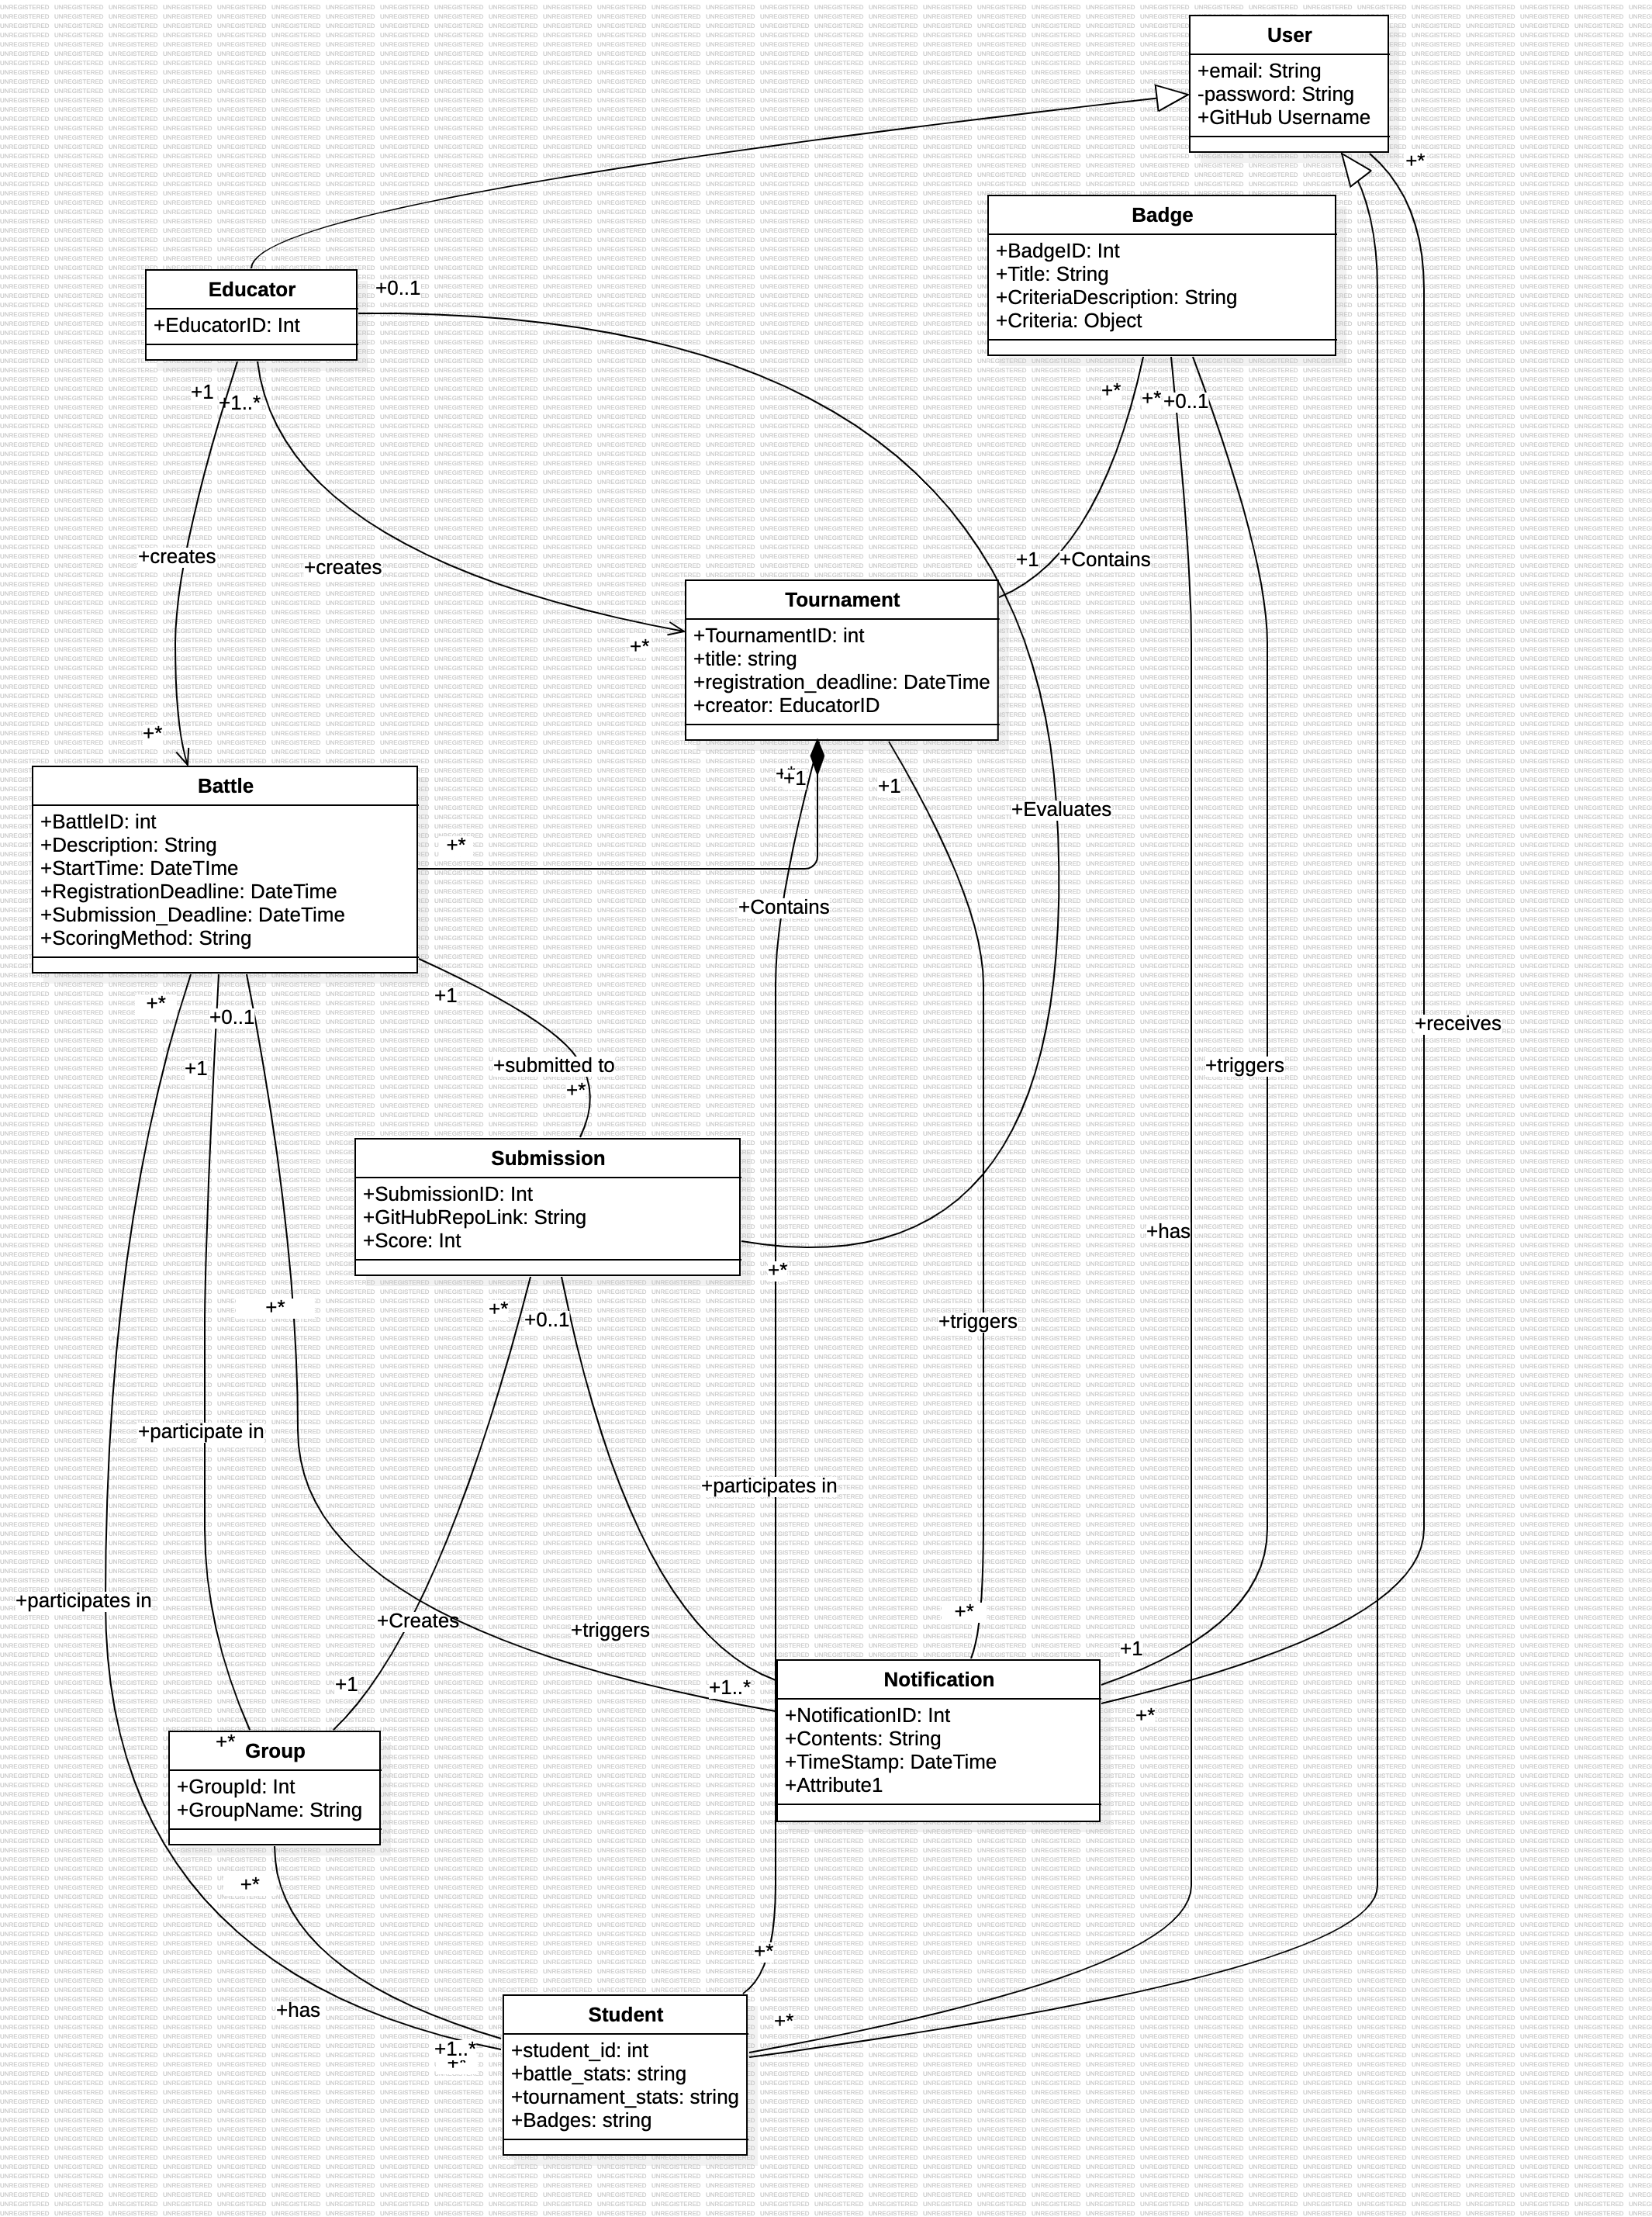
\includegraphics[width=\textwidth]{Graphics/Main.png}
    \caption{UML Domain Class Diagram}
    \label{fig:ClassDiagram}
\end{figure}


\subsection{State charts}

These two state diagrams gives an overview over the two most essential process within CodeKataBattles, namely the Battle and Tournament. 

\begin{figure}[htbp]
    \centering
    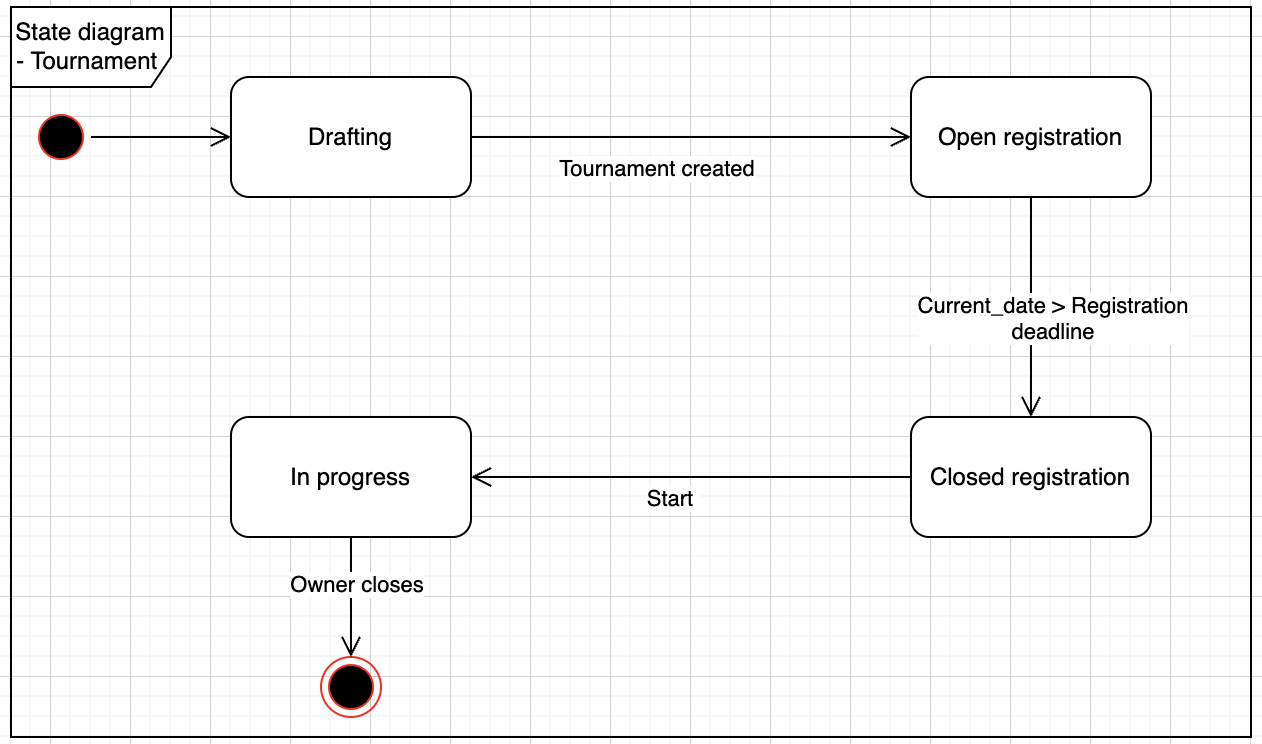
\includegraphics[width=\textwidth]{Graphics/State Diagram/Tournament.png}
    \caption{State Diagram - Tournament}
    \label{fig:TStateDiagram}
\end{figure}
Figure \ref{fig:TStateDiagram} shows the progression of a tournament in CodeKataBattles. Initiated by an educator, the "Drafting" phase involves filling in the tournament's details such as the title and registration deadline. Once established, the system transitions the tournament to "Open registration," allowing students to join until the deadline, after which it moves to "Closed registration." When the start date is surpassed, the tournament enters the "In progress" stage, which is where the battle can be had. This continues until the educator decides to end the event, bringing the tournament to its end and finalizing the standings.
\begin{figure}[htbp]
    \centering
    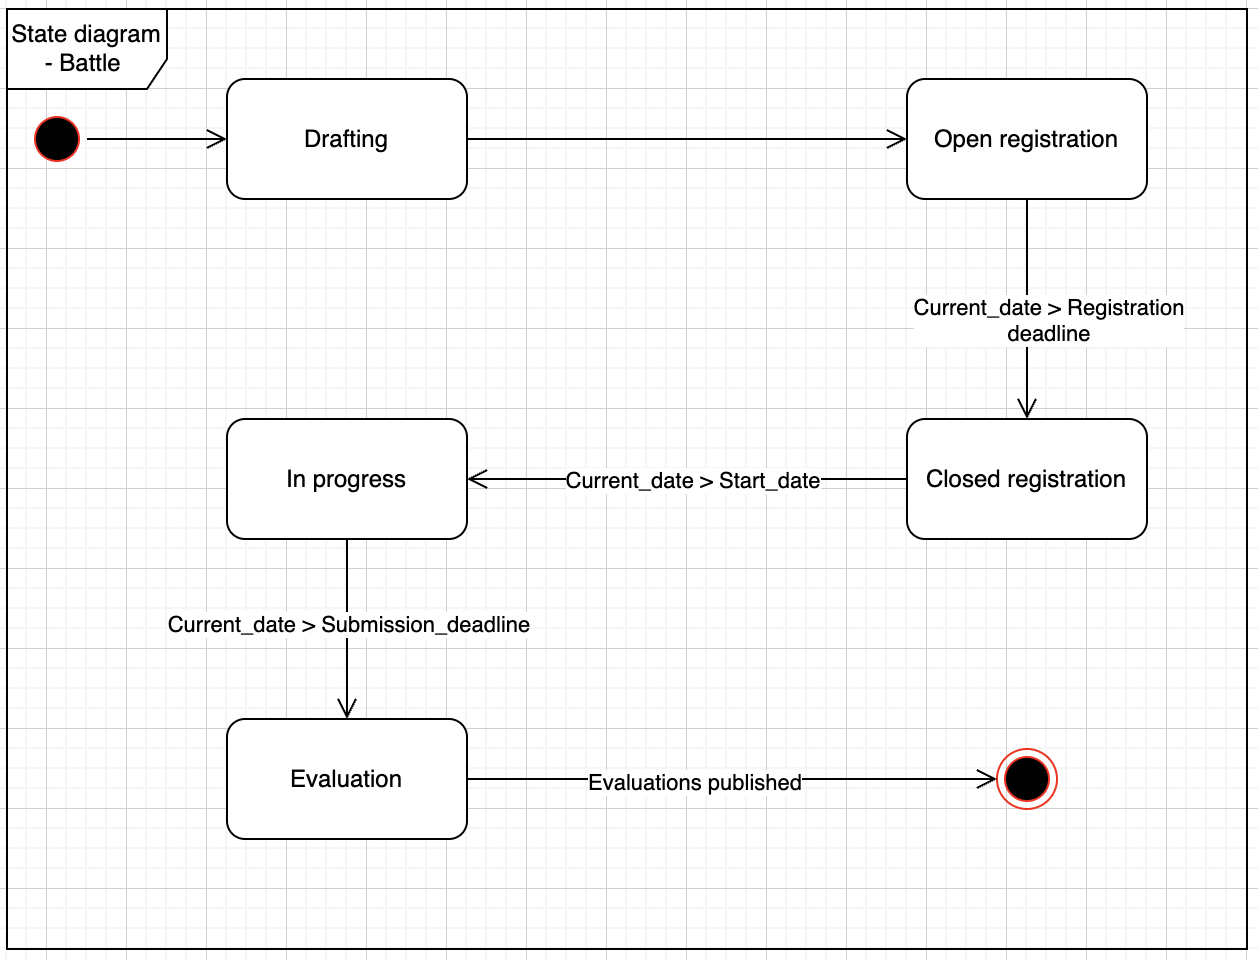
\includegraphics[width=\textwidth]{Graphics/State Diagram/Battle.png}
    \caption{State Diagram - Battle}
    \label{fig:BStateDiagram}
\end{figure}

Figure \ref{fig:BStateDiagram} displays the lifecycle of a battle within CodeKataBattles. A battle initial state the "Drafting" starts when an educator decides to create a battle within a tournament. Here the educator details the deadlines, the title, the description, and the automation scripts containing the test cases. Once that is done, and the battle's details are validated by the system, the battle is created and precedes to be open for registration. Here students within the tournament can in teams of 1 or more join the battle, however, once the registration deadline is passed the battle is closed for registrations. This waiting state is over when the start date of the battle is surpassed, commencing the "in progress" stage of the battle. Here students can submit as many solutions for the problem and get feedback. The stage ends when the submission deadline is finished. Now all the team's best solutions are put into the final ranking, and every participant in the battle is notified. Hereafter the Battle has ended.  
\subsection{Product functions}

The following section will have a detailed description of the CodeKataBattles functions. 


\begin{enumerate}
    \item {\textbf{Sign-Up \& Log In}}\newline
    This functionality should enable the user to register as a user on the platform. Each user has to specify their email and their GitHub username. We will use the email as their username, and let them specify their passwords under standard security requirements. For the user to finalize their registration, and verification email is sent to the given email with a link for the user to confirm their access to the email. After the initial sign-up process is finished, the user can log on to the platform via their specified email and password. 
    \item {\textbf{Create battle}}\newline
    Available to every educator is the ability to create a battle under a given tournament, where the educator has the required permissions. The educator then needs to specify a number of elements to finalize the creation of the battle. One element concerns the technical documents making up the code kata. Here the educator is required to specify a description of the battle, test cases specifying how a satisfactory solution should behave, and lastly include the automation scripts. Thereafter the educator has to make the formal configuration of the code kata, which entails setting the minimum and maximum size of the groups and setting the registration and final submission deadline. The last element to specify is the configuration of the scoring methodology for the battle. Here the educator can enable manual scoring or automate the process in a weighted manner to their liking. 
    \item {\textbf{Join battle}}\newline
    Students can see the tournaments open for registration, and the open battles, in tournaments they already have joined. When selecting to join a battle, the user is prompted to create a group. The group can consist of the sole creator of the group, or the student can invite as many additional students as the battle allows. The other students need to already be registered for the tournament to be able to be invited. Each group needs a name unique to the battle participants. 
    \item {\textbf{Create tournament}}\newline
    Only an educator can create a tournament. A tournament requires a title, registration deadline, and specification of badges for the tournament. Each badge needs a title, and a set of rules enabling the automation of giving out the badge to participants that fulfill the requirements for the badge. Beyond the registration deadline putting a threshold of when students can join the battle, the deadline also constrains battle deadlines in the tournaments to be after the battle. To enable other educators to create battles within the tournament, the original creator of the tournament has to add the educator by username to a list of educators with permission. 
    \item {\textbf{Receive Notifications from battles}}\newline
    When a student or group has joined a battle they are placed on a notification list that enables them to receive notifications in several scenarios:
    \begin{enumerate}
        \item When the registration deadline is transgressed users receive a link to the GitHub repository containing code descriptions, build automation scripts, and other relevant files. 
        \item When a submission has been evaluated the user receives a notification containing indexes of the tests that the program has passed as well as the score for the solution.
        \item When the submission deadline is transgressed the user receives a notification with the final score and rank in the battle.
    \end{enumerate}
    \item {\textbf{Receive Notifications from Tournaments}}\newline
    If a user is subscribed to a tournament the user is placed on a notification list so they can be notified in certain situations. The user is notified when a battle is created under a tournament. The user is notified of their tournament rank \& score when the tournament is ended by a permitted educator. The user is notified if they qualify for any badges specified in the tournament. 
    \item {\textbf{See tournament information}}\newline
    In order to keep up with their performance and upcoming battles, users can inspect Tournament information. This includes seeing previous, future, and ongoing battles of the tournaments along with relevant summary statistics, such as average score and number of participants. Additionally, the user can see their current rank and score on the tournament leaderboard. Users can also inspect if they have received any badges in the tournament. 
    \item {\textbf{See battle information}}\newline
    This functionality allows users to keep up with the battles they are involved in. This includes seeing the attempts made by the user or group along with the number of tests passed by each attempt. The battle leaderboard reveals the rank and score of the user or group in the current battle. The information on remaining time until the submission deadline and the number of participants is also visible.

    \item {\textbf{Display Student Profile}}\newline
    This functionality allows students and educators to view student's battle and tournament involvement. This includes rankings, badges and achievements. 
\end{enumerate}

\subsection{User characteristics}
The CodeKataBattles system is primarily interacted with by two categories of users: Students and Educators.

\subsubsection{Student}
In the context of CodeKataBattles, a student is a type of user registered on the CodeKataBattle platform solely for participating in code kata battles and tournaments. They cannot create battles or tournaments. They have a device with an internet browser and internet connection so they can access the web application. 

\subsubsection{Educator}
In the context of CodeKataBattles, an educator is a type of user registered on the CodeKataBattle platform for creating and hosting tournaments in code kata battles and tournaments. They can also score submissions in battles where manual evaluation is enabled and she/he is owner of the tournament. They can also close down tournaments at will.
They have a device with an internet browser and internet connection so they can access the web application. 


\subsection{Assumptions, dependencies and constraints}

\subsubsection{Regulatory Policies}
The CodeKataBattle platform will ask for user personal information like email address linked with a GitHub user. Email addresses and Github user information won’t be used for commercial purposes. Personal information will be processed in compliance with the GDPR.


\subsubsection{Domain Assumptions}
\label{sec:domain_assumptions}

This section outlines the assumptions that are considered as given within the operational domain of the CodeKataBattle system. These are conditions that the system presumes to be true and are necessary for the correct operation and use of the platform.

\begin{enumerate}
    \item \textbf{[D1]} Users must have a stable internet connection to access and interact with the CodeKataBattle platform.
    \item \textbf{[D2]} Users' computing devices must be capable of running the necessary software development tools for coding battles.
    \item \textbf{[D3]} GitHub services are available and reliable as the platform depends on GitHub for repository hosting and Actions for automated workflows.
    \item \textbf{[D4]} Educators and students must have a basic understanding of how to use version control systems, particularly GitHub.
    \item \textbf{[D5]} Automated testing scripts provided in code katas are correct and capable of accurately evaluating the students' code submissions.
    \item \textbf{[D6]} Users must allow notification services to receive timely updates from the CodeKataBattle platform.
    \item \textbf{[D7]} The static analysis tools integrated with the platform for code quality assessment are functioning and accessible.
    \item \textbf{[D8]} Students' submissions through GitHub are timestamped accurately to ensure fair evaluation of timeliness.
    \item \textbf{[D9]} Educators inputting the battle information, including test cases and scoring configurations, must ensure their accuracy and clarity.
    \item \textbf{[D10]} The computing environment used by students for development is compatible with the code kata requirements and specifications.
    \item \textbf{[D11]} The system's timekeeping is synchronized with an accurate time source to ensure deadline enforcement.
    \item \textbf{[D12]} Educators are responsible for defining clear and measurable objectives for battles and tournaments.
    \item \textbf{[D13]} Students are expected to follow the test-first approach as specified in the battle requirements, creating tests before implementation.
    \item \textbf{[D14]} Scores and feedback are assumed to be constructive and used for educational purposes, not as punitive measures.
    \item \textbf{[D15]} The platform assumes all users act in good faith, not attempting to game the system or manipulate scores through unfair means.
\end{enumerate}


\newpage
\clearpage
\newpage
\section{Specific Requirements}
\label{sec:reqs}
%include more details on all aspects of section 2 if they are useful for the development team

\subsection{External Interface Requirements}
\subsubsection{User Interfaces}
This section presents the user interfaces for the CodeKataBattles platform. The first section is dedicated to the user interfaces encountered by the student, and the second section to those encountered by the educator. While similar on many accounts as both students and educators need the ability to monitor and receive notifications about relevant tournaments and battles. However, students' interactions with battles and tournaments are limited to monitoring and subscribing, while educators can create new battles and tournaments. While the service needs to be accessed by a heterogeneous set of users, because a lot of the intricacies of the difference in use-cases are handled by GitHub, a lot of the functionalities available to students and educators are very closely related. 

\newpage
\clearpage
\subsection{Students}

\begin{figure}[Htbp!]
    \centering
    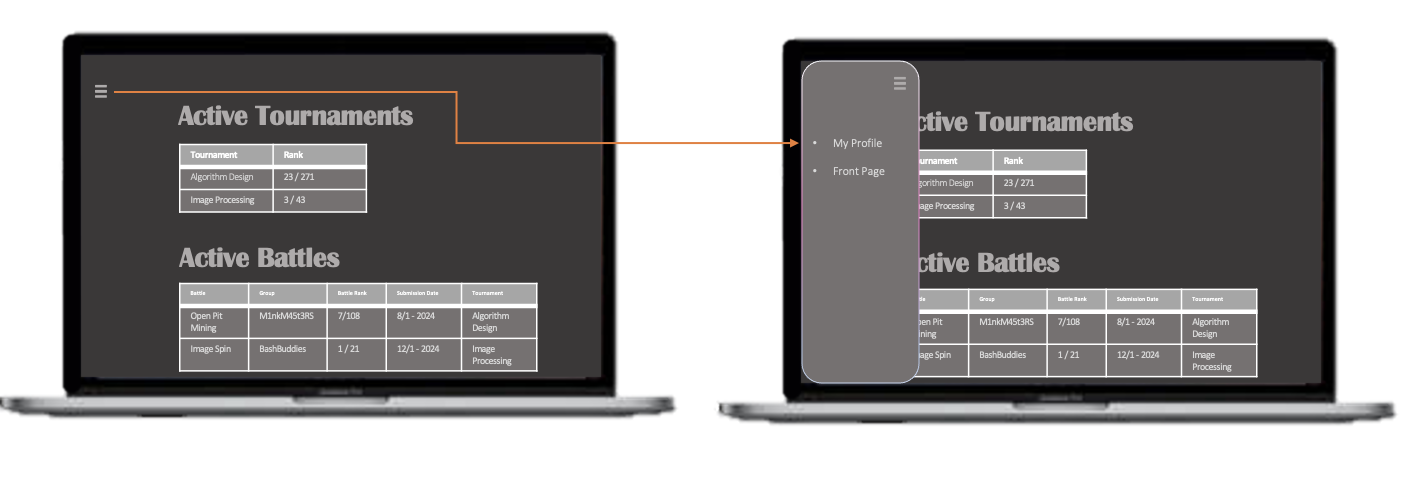
\includegraphics[width=\textwidth]{Graphics/SIDE BAR.png}
    \caption{User Interface: Front Page \& Sidebar}
    \label{fig:Sidebar}
\end{figure}

\begin{figure}[Htbp!]
    \centering
    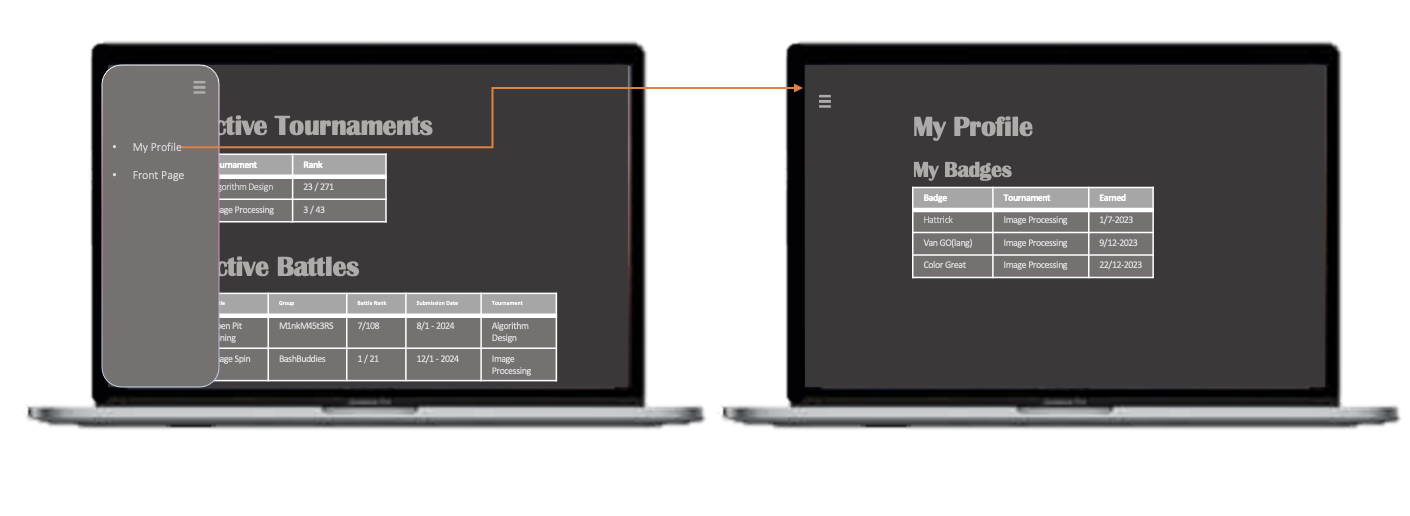
\includegraphics[width=\textwidth]{Graphics/MY PROFILE.png}
    \caption{User Interface: Profile}
    \label{fig:profile}
\end{figure}

\begin{figure}[Htbp!]
    \centering
    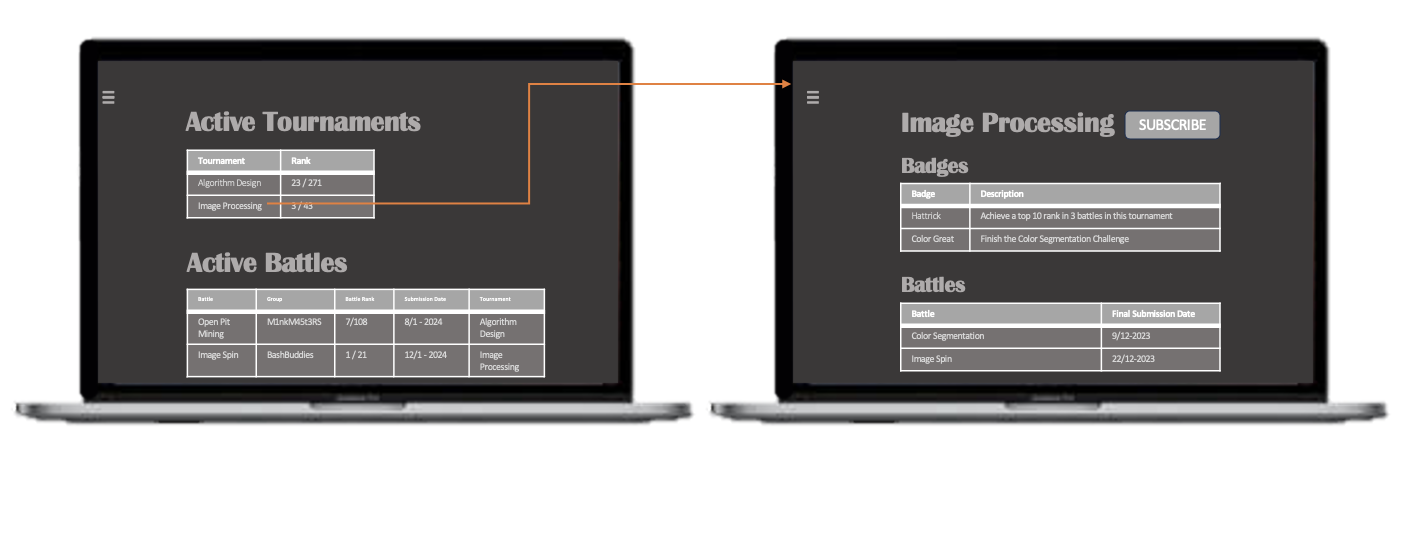
\includegraphics[width=\textwidth]{Graphics/TOURNAMENTS.png}
    \caption{User Interface: Tournament Page}
    \label{fig:tournaments}
\end{figure}


\begin{figure}[Htbp!]
    \centering
    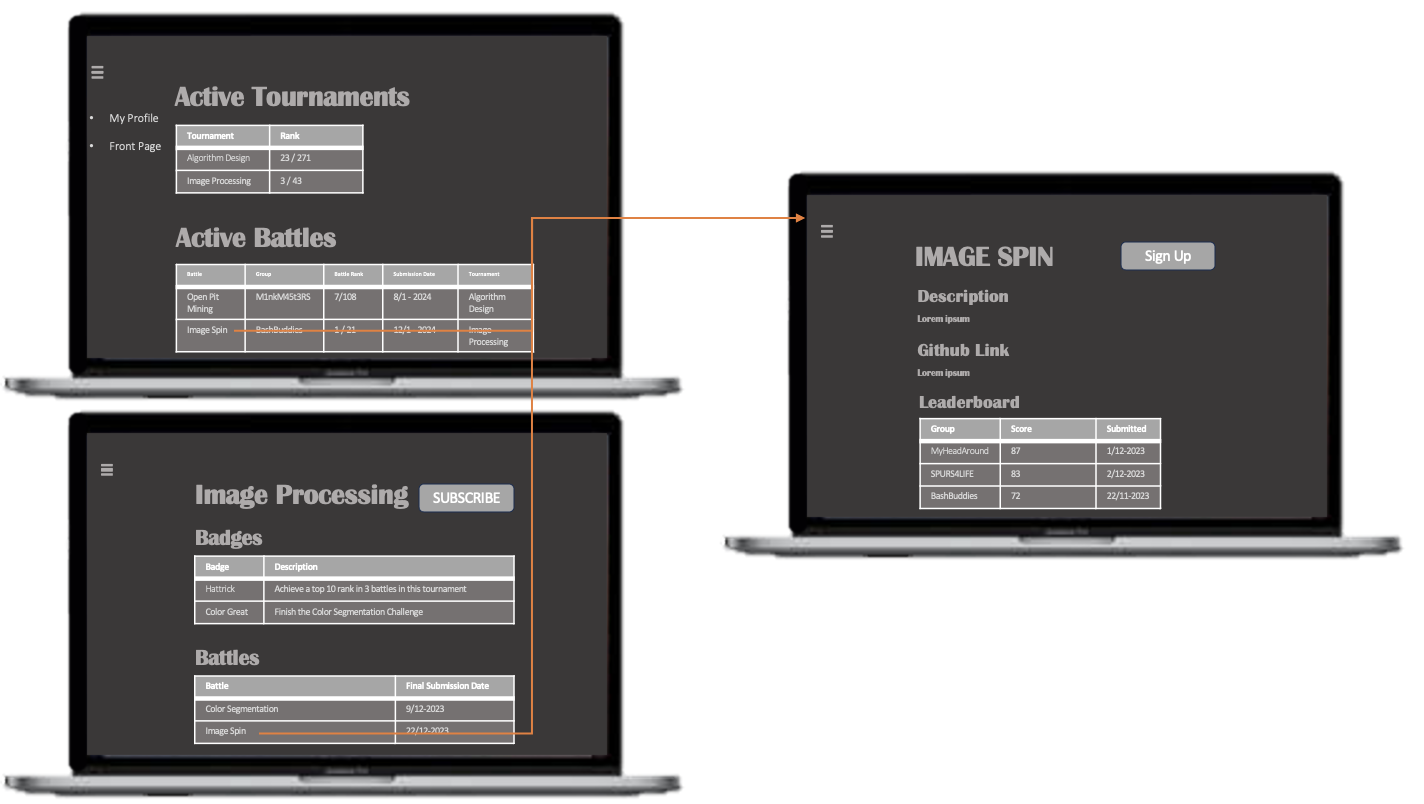
\includegraphics[width=\textwidth]{Graphics/BATTLE.png}
    \caption{User Interface: Battle Page}
    \label{fig:battle}
\end{figure}


\begin{figure}[Htbp!]
    \centering
    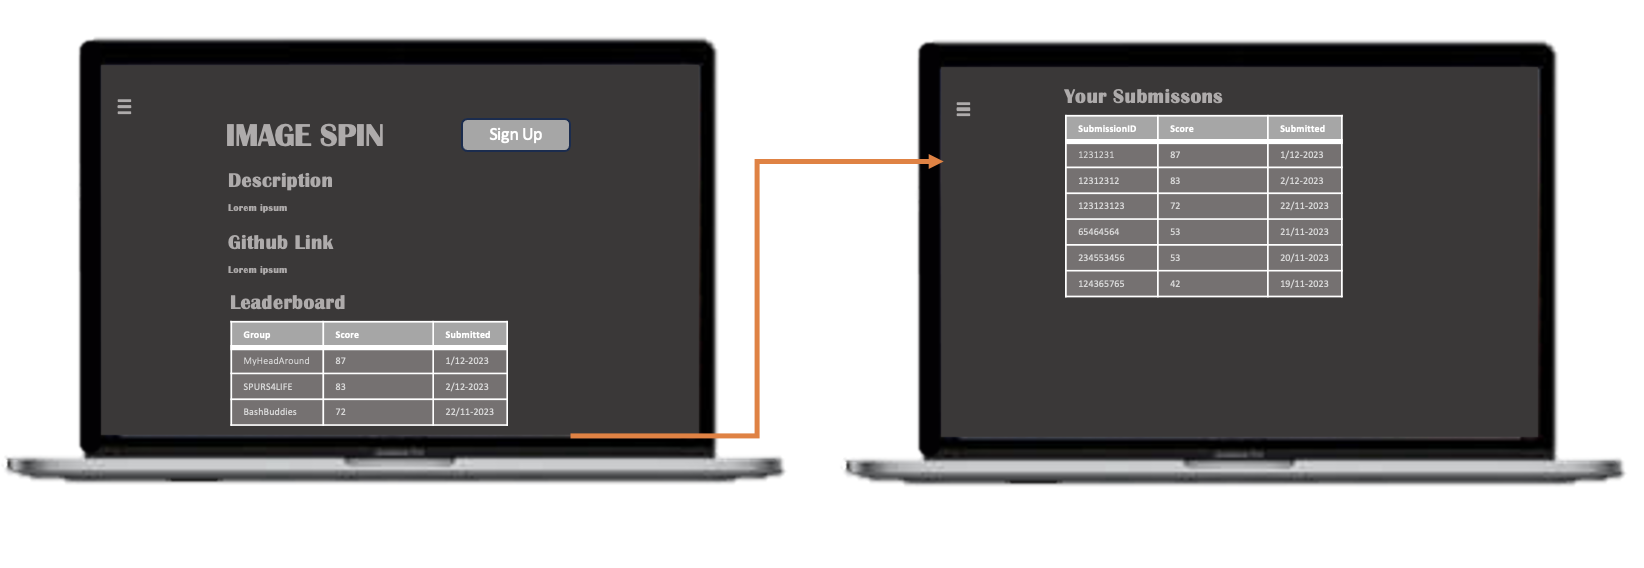
\includegraphics[width=\textwidth]{Graphics/SUBMISSION LOG.png}
    \caption{User Interface: Battle Page (Submission Log)}
    \label{fig:submissionlog}
\end{figure}

\subsection{Educators}

\begin{figure}[Htbp!]
    \centering
    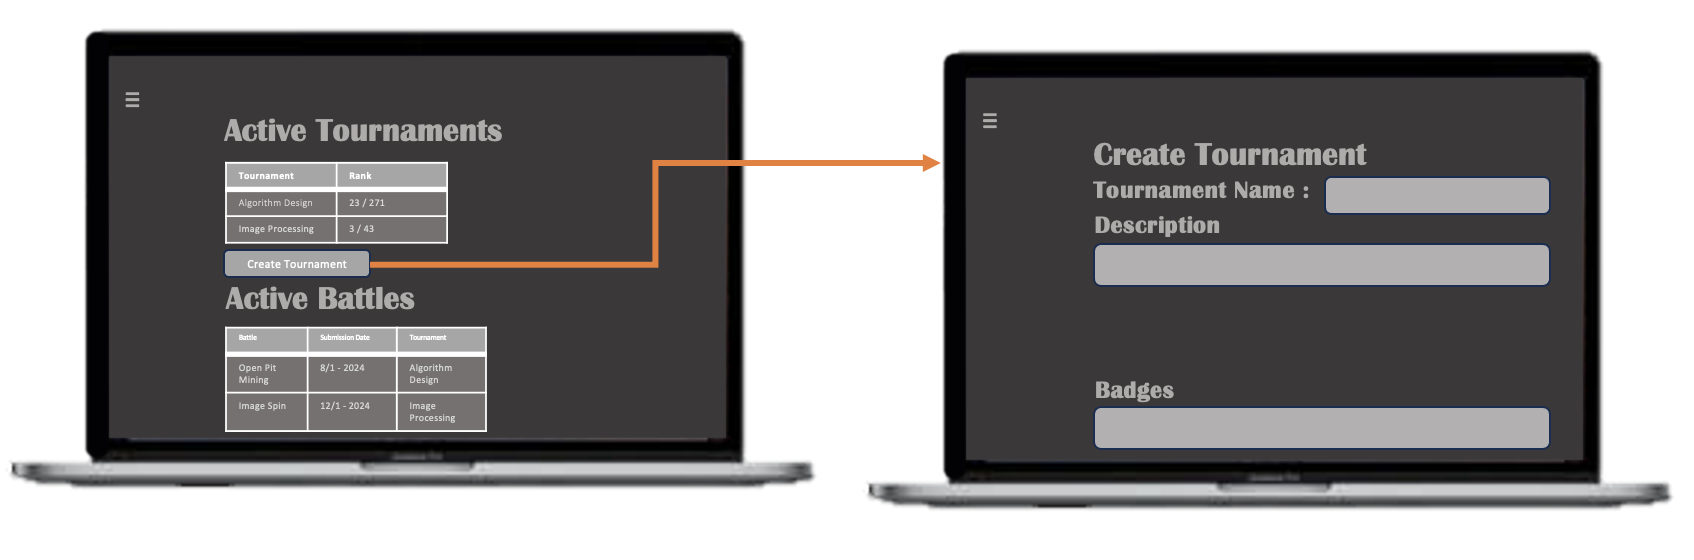
\includegraphics[width=\textwidth]{Graphics/CREATE TOURNAMENT.png}
    \caption{User Interface: Create Tournament Page}
    \label{fig:createTournament}
\end{figure}


\begin{figure}[Htbp!]
    \centering
    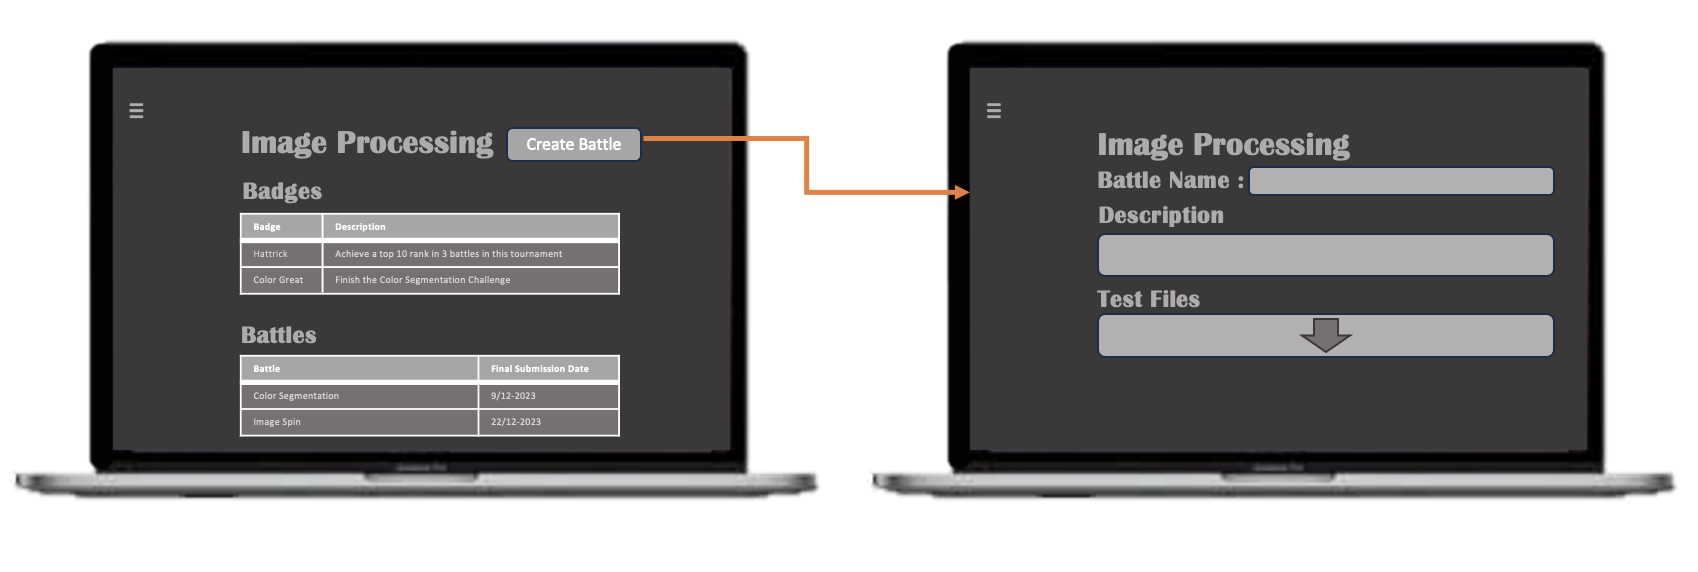
\includegraphics[width=\textwidth]{Graphics/CREATE BATTLE.png}
    \caption{User Interface: Create Battle Page}
    \label{fig:createBattle}
\end{figure}


\subsubsection{Hardware Interfaces}
All users, both Students and Educators can access the platform through a web browser. Therefore, all users need access to a device with an internet connection and browser installed. While note strictly required, a text editor is also recommended. 

\subsubsection{Software Interfaces}
The system utilizes one primary external service, namely Github. A Github action is set up, such that any pushes to a forked repository from a given battle is automatically pulled by the system. Then a predefined test script evaluates the implementation on a variety of tests.  

\subsection{Functional Requirements}
\label{sec:functional_requirements}

The CodeKataBattle system is designed to facilitate and manage competitive coding exercises, known as code katas. The system shall support the following functional requirements to ensure a comprehensive and engaging learning experience for students:

\begin{enumerate}
    \item \textbf{[R1]} The system shall allow users to sign up using their GitHub credentials (i.e. their email and GitHub Username).
    \item \textbf{[R2]} The system shall send a verification email to confirm a user's account upon sign-up.
    \item \textbf{[R3]} Educators shall be able to create tournaments with a specified title.
    \item \textbf{[R4]} Educators shall be able to set registration deadlines for tournaments.
    \item \textbf{[R5]} Educators shall be able to define tournament badge criteria.
    \item \textbf{[R6]} The system shall notify users of new tournaments.
    \item \textbf{[R7]} Users shall be able to subscribe to tournaments by a given deadline.
    \item \textbf{[R8]} Educators shall be able to create battles within tournaments.
    \item \textbf{[R9]} Educators shall be able to upload technical documents for battles.
    \item \textbf{[R10]} Educators shall be able to set the minimum and maximum number of students per group for battles.
    \item \textbf{[R11]} Educators shall be able to set a registration deadline for battles.
    \item \textbf{[R12]} Educators shall be able to set a final submission deadline for battles.
    \item \textbf{[R13]} Educators shall be able to configure scoring methodologies for battles.
    \item \textbf{[R14]} Students shall be able to form teams to join battles.
    \item \textbf{[R15]} The system shall provide a GitHub repository link for the code kata to registered teams after the registration deadline.
    \item \textbf{[R16]} The system shall automatically score submissions based on the results of test cases.
    \item \textbf{[R17]} The system shall evaluate the timeliness of submissions.
    \item \textbf{[R18]} The system shall assess the quality level of source code through static analysis.
    \item \textbf{[R19]} Educators shall have the option to manually score submissions.
    \item \textbf{[R20]} The system shall update battle scores in real-time upon new commits on GitHub.
    \item \textbf{[R21]} The system shall notify participants of final battle ranks after the consolidation phase.
    \item \textbf{[R22]} The system shall update personal tournament scores with the sum of battle scores.
    \item \textbf{[R23]} The system shall maintain a visible tournament rank for each student.
    \item \textbf{[R24]} Educators shall be able to define gamification badges with specific rules.
    \item \textbf{[R25]} The system shall display badges on student profiles.
    \item \textbf{[R26]} Educators shall be able to close tournaments and trigger final rank notifications.
    \item \textbf{[R27]} The system shall enable boolean expressions to define rules of badges and achievements.
    \item \textbf{[R28]} Students shall be able to visualize their performance.
    \item \textbf{[R29]} Students shall be able to visualize their tournament information.
    \item \textbf{[R30]} Students shall be able to track their battle involvement.
    \item \textbf{[R31]} Students shall be able to see detailed logs of their attempt outcomes.
\end{enumerate}

Definition of use case diagrams, use cases and associated sequence/activity diagrams, and mapping on requirements
 
\subsection{Performance Requirements}
\label{sec:performance_requirements}
The CodeKataBattles platform, recognizing the unique nature of code kata activities, has tailored performance requirements, especially concerning system downtime. Since a substantial part of the participation occurs in personal text editors or IDEs, the platform can accommodate longer downtimes without significantly impacting user productivity. An accepted downtime of up to half an hour is considered reasonable, allowing users to continue their work offline during such periods.

To minimize disruption, scheduled maintenance is planned during off-peak hours, and users are notified in advance through various channels. In case of unexpected downtimes, prompt communication is ensured, providing users with information and an estimated resolution time. Despite this tolerance for downtime, ensuring data integrity remains paramount. The platform is equipped with robust backup mechanisms to safeguard user data and maintain accessibility after downtimes.

These performance requirements reflect a balance between user experience and the practicalities of system maintenance for CodeKataBattles, catering to the platform's specific workflow.




\subsection{Design Constraints}

\subsubsection{Standards compliance}
Regarding data privacy, the CKB platform adheres to the General Data Protection Regulation (GDPR), which governs data protection and privacy for individuals within the European Union (EU) and the European Economic Area (EEA). Additionally, the system must comply with international standards for using and representing dates and times.

\subsubsection{Hardware limitations}
Here we report relevant hardware requirements. The only real hardware requirement is a machine with an Internet connection (2G/3G/4G/Wi-Fi) and a modern web browser

\subsection{Software System Attributes}
\subsubsection{Reliability}
As mentioned in section \ref{sec:performance_requirements} this service does not warrant complex infrastructure to aggressively reduce downtime, due to the amount of work being done in text editors or IDEs not directly connected to the platform. This is also the case for data, as all code is stored in Github repositories, however, all data related to the gamification aspect of the platform is stored only in the system. 

\subsubsection{Security}
As for any system handling personal information, such as CodeKataBattles does with information regarding educators and students, security is vital. 
To ensure compliance with security standards, encryption of passwords within the database must be applied. The same encryption need is present for data in transmission over the internet, to avoid interception-tactics. User's access to data must be a constraint to information deemed relevant for them through the use of role-based access control. 

\subsubsection{Availability}
CodeKataBattles is not a critical service, so the availability role is mainly to create a good user experience. Furthermore as mentioned in \ref{sec:performance_requirements} user productivity can exist in downtime. Therefore the system should aim to provide at least 99\% availability, meaning that the average time between occurrences of a failure and
service recovery (MTTR) must be less or equal to 3,65 days per year. 

\subsubsection{Maintainability}
The system is required to ensure a high level of maintainability. This entails the utilization of appropriate design patterns and adherence to recognized coding standards. The code must be well-documented, and practices such as hard-coding are strictly avoided. Moreover, the system should include a comprehensive testing routine, which is expected to cover a minimum of 75\% of the entire codebase, with the exception of interface code.

\subsubsection{Portability}
The web application should be compatible with all operating systems that support a web browser, including Windows, macOS, Linux, and others.

\begin{table}[h!]
\centering
\begin{tabular}{|p{0.2\textwidth}|p{0.7\textwidth}|}
\hline
\textbf{Name} & Login User \\
\hline
\textbf{Actors} & Student \& educator \\
\hline
\textbf{Entry Condition} & The student/educator has opened the CodeKata web application \\
\hline
\textbf{Event flow} & 
\begin{minipage}[t]{0.7\textwidth}
1 - The user inserts his username and password in the form \\
2 - The user clicks on the “Login” button \\
3 - The system checks the credentials \\
4 - The application shows the proper dashboard
\end{minipage} \\
\hline
\textbf{Exit condition} & The user has access to the services for the right interface provided by the CodeKata web application \\
\hline
\textbf{Exception} & 
\begin{minipage}[t]{0.7\textwidth}
3 - The data inserted are not valid. The system returns to the entry condition.
\end{minipage} \\
\hline
\end{tabular}
\caption{Use Case Specification}
\end{table}


\begin{table}[h!]
\centering
\begin{tabular}{|p{0.2\textwidth}|p{0.7\textwidth}|}
\hline
\textbf{Name} & Join tournament \\
\hline
\textbf{Actors} & Student \\
\hline
\textbf{Entry Condition} & 
\begin{minipage}[t]{0.7\textwidth}
1 - The student is logged into the CodeKata platform \\
2 - The student is on the home page of the CodeKata web application \\
3 - The registration deadline has not yet passed
\end{minipage} \\
\hline
\textbf{Event flow} & 
\begin{minipage}[t]{0.7\textwidth}
1 - The student selects one of the available tournaments on the homepage \\
2 - The student clicks on the “Join” button \\
3 - The system adds the specific user to the participant list for the given tournament \\
4 - The tournament is added to the overview of tournaments the student is currently participating in
\end{minipage} \\
\hline
\textbf{Exit condition} & 
The student now has access to the battles within the tournament and is returned to the tournament home page \\
\hline
\textbf{Exception} & \\
\hline
\end{tabular}
\caption{Use Case Specification}
\end{table}


\begin{table}[h!]
\centering
\begin{tabular}{|p{0.2\textwidth}|p{0.7\textwidth}|}
\hline
\textbf{Name} & Join battle \\
\hline
\textbf{Actors} & Student \\
\hline
\textbf{Entry Condition} & 
\begin{minipage}[t]{0.7\textwidth}
1 - The student is logged in \\
2 - The student is subscribed to the tournament, to which the battle belongs \\
3 - The battle is open for registration \\
4 - The student resides on the battles page
\end{minipage} \\
\hline
\textbf{Event flow} & 
\begin{minipage}[t]{0.7\textwidth}
1 - The student clicks on the “Join” button \\
2 - The student is prompted to specify participant(/s) by username in its group \\
3 - The student enters the name of the group \\
4 - The system adds the specific user/team to the participant list for the given battle \\
5 - The battle is added to the overview of battles the student is currently participating in
\end{minipage} \\
\hline
\textbf{Exit condition} & 
The student will now receive notifications relevant to the given battle and is returned to the battle's home page \\
\hline
\end{tabular}
\caption{Use Case Specification}
\end{table}




% Skal lige kigges over de her tables 
\begin{table}[h!]
\centering
\begin{tabular}{|l|l|}
\hline
\textbf{Name} & Create Battle \\
\hline
\textbf{Actors} & Educator \\
\hline
\textbf{Entry Condition} & 
\begin{tabular}[c]{@{}l@{}}
1 - The educator is logged into the CodeKata platform. \\
2 - The educator has the details of a specific tournament displayed. \\
\end{tabular} \\
\hline
\textbf{Event flow} & 
\begin{tabular}[c]{@{}l@{}}
1 - The educator clicks the “Create Battle” button. \\
2 - The educator uploads a brief textual description of the battle. \\
3 - The educator uploads a software project with build automation scripts. \\
4 - The educator sets the registration and submission deadlines. \\
5 - The educator selects the scoring methodology. \\
6 - The system confirms the creation of the battle. \\
\end{tabular} \\
\hline
\textbf{Exit condition} & 
The battle is created, enabling educator management within the tournament.\\
\hline
\textbf{Exception} & 
\begin{tabular}[c]{@{}l@{}}
If required details are missing or incorrect, the educator is prompted for correction. \\
\end{tabular} \\
\hline
\end{tabular}
\caption{Use Case Specification for Creating a Battle}
\end{table}

\begin{table}[h!]
\centering
\begin{tabular}{|l|l|}
\hline
\textbf{Name} & Manual Battle Evaluation \\
\hline
\textbf{Actors} & Educator \\
\hline
\textbf{Entry Condition} & 
\begin{tabular}[c]{@{}l@{}}
1 - The educator is logged in. \\
2 - The educator is the owner of the battle. \\
3 - The submission deadline for the battle has passed. \\
\end{tabular} \\
\hline
\textbf{Event flow} & 
\begin{tabular}[c]{@{}l@{}}
1 - The educator navigates to the battle's submission list. \\
2 - The educator selects a submission for review. \\
3 - The educator assesses the submission, assigning a manual score. \\
4 - The system updates the battle's rankings with the new score. \\
4 - The system notifies the creator/s of the submissions of evaluation. \\ %skal det her være en exit condition?
\end{tabular} \\
\hline
\textbf{Exit condition} & 
The evaluated submission has been scored and displayed in the battle's rankings. \\
\hline
\textbf{Exception} & 
\begin{tabular}[c]{@{}l@{}}
If an error occurs during scoring, the educator is notified to retry. \\
\end{tabular} \\
\hline
\end{tabular}
\caption{Use Case Specification for Evaluating a Submission}
\end{table}



\begin{table}[h!]
\centering
\begin{tabular}{|l|l|} 
\hline
\textbf{Name} & Create a Badge \\
\hline
\textbf{Actors} & Educator \\
\hline
\textbf{Entry Condition} & 
\begin{tabular}[c]{@{}l@{}}
1 - The educator is logged into the CodeKata platform. \\
2 - The educator is the creator of the tournament. \\
\end{tabular} \\
\hline
\textbf{Event flow} & 
\begin{tabular}[c]{@{}l@{}}
1 - The educator selects the option to create a new badge. \\
2 - The educator inputs the badge name, description, and criteria. \\
3 - The system validates the input and creates the badge. \\
\end{tabular} \\
\hline
\textbf{Exit condition} & 
A new badge is created and available for awarding to students in the tournament. \\
\hline
\textbf{Exception} & 
\begin{tabular}[c]{@{}l@{}}
If the criteria are not valid, the educator is prompted to correct the information. \\
\end{tabular} \\
\hline
\end{tabular}
\caption{Use Case Specification for Creating a Badge}
\end{table}

\begin{table}[h!]
\centering
\begin{tabular}{|l|l|}
\hline
\textbf{Name} & Check Tournament Ranking \\
\hline
\textbf{Actors} & Student \\
\hline
\textbf{Entry Condition} & 
\begin{tabular}[c]{@{}l@{}}
1 - The student is logged into the CodeKata platform. \\
2 - The student is participating in the tournament. \\
\end{tabular} \\
\hline
\textbf{Event flow} & 
\begin{tabular}[c]{@{}l@{}}
1 - The student navigates to the tournament overview. \\
2 - The student selects the tournament to view. \\
3 - The system displays the current ranking and score of all participants. \\
\end{tabular} \\
\hline
\textbf{Exit condition} & 
The student views their current standing within the tournament rankings. \\
\hline
\textbf{Exception} & 
\begin{tabular}[c]{@{}l@{}}
If the rankings are not available, the battle's start time is yet to be surpassed. \\
\end{tabular} \\
\hline
\end{tabular}
\caption{Use Case Specification for Checking Tournament Ranking}
\end{table}

\begin{table}[h!]
\centering
\begin{tabular}{|l|l|}
\hline
\textbf{Name} & Automatic Scoring of a Submission \\
\hline
\textbf{Actors} & System \\
\hline
\textbf{Entry Condition} & A group has submitted their solution. \\
\hline
\textbf{Event flow} & 
\begin{tabular}[c]{@{}l@{}}
1 - The system retrieves the latest commit from the group's GitHub repository. \\
2 - The system runs automated tests against the submission. \\
3 - The system calculates the score based on the test results. \\
4 - The system updates the battle's leaderboard with the new score. \\
\end{tabular} \\
\hline
\textbf{Exit condition} & 
The group's submission is scored and the leaderboard reflects the updated score. \\
\hline
\textbf{Exception} & 
\begin{tabular}[c]{@{}l@{}}
Errors during test execution or score calculation prompt system retry. \\
\end{tabular} \\
\hline
\end{tabular}
\caption{Use Case Specification for Automatic Scoring of a Submission}
\end{table}

\begin{table}[h!]
\centering
\begin{tabular}{|l|l|}
\hline
\textbf{Name} & Announcing Tournament Results \\
\hline
\textbf{Actors} & System \\
\hline
\textbf{Entry Condition} & 
\begin{tabular}[c]{@{}l@{}}
1 - All battles' submission deadlines within the tournament have passed.\\
2 - The tournament creator clicks the button on the tournament page to end it.  \\
\end{tabular} \\
\hline
\textbf{Event flow} & 
\begin{tabular}[c]{@{}l@{}}
1 - The system compiles final scores from all tournament battles. \\
2 - The system determines tournament winners and badge recipients. \\
3 - The system sends notifications to participants with final standings. \\
4 - The system updates the tournament page with the final results. \\
\end{tabular} \\
\hline
\textbf{Exit condition} & 
Participants get final results; standings are shown on the tournament page. \\
\hline
\textbf{Exception} & 
\begin{tabular}[c]{@{}l@{}}
Failure in result compilation or notification delivery triggers a retry. \\
\end{tabular} \\
\hline
\end{tabular}
\caption{Use Case Specification for Announcing Tournament Results}
\end{table}

\begin{table}[h!]
\centering
\begin{tabular}{|l|l|}
\hline
\textbf{Name} & View Tournament Ranking \\
\hline
\textbf{Actors} & Student, Educator \\
\hline
\textbf{Entry Condition} & 
The user is logged into the CodeKata platform and participating in a tournament. \\
\hline
\textbf{Event flow} & 
\begin{tabular}[c]{@{}l@{}}
1 - The user navigates to the specific tournament section. \\
2 - The user selects the option to view rankings. \\
3 - The system displays the leaderboard with student names and scores. \\
4 - User reviews the ranking positions and individual scores. \\
\end{tabular} \\
\hline
\textbf{Exit condition} & 
The user views their tournament ranking and scores. \\
\hline
\textbf{Exception} & 
\begin{tabular}[c]{@{}l@{}}
If the leaderboard isn't updated, the system suggests a page refresh. \\
\end{tabular} \\
\hline
\end{tabular}
\caption{Use Case Specification for Viewing Tournament Ranking}
\end{table}

\begin{table}[h!]
\centering
\begin{tabular}{|l|l|}
\hline
\textbf{Name} & Push a new commit to a battle solution\\
\hline
\textbf{Actors} & Student \\
\hline
\textbf{Entry Condition} & 
\begin{tabular}[c]{@{}l@{}}
1 - The student is logged into the CodeKata platform. \\
2 - The student is part of a group in an ongoing battle. \\
\end{tabular} \\
\hline
\textbf{Event flow} & 
\begin{tabular}[c]{@{}l@{}}
1 - The student updates their submission, by pushing a new commit in the forked GitHub repository. \\
2 - The system validates the submission and confirms receipt. \\
3 - The system queues the submission for scoring. \\
\end{tabular} \\
\hline
\textbf{Exit condition} & 
Submission is successfully uploaded and awaiting evaluation. Automatic submission evaluation is triggered. \\
\hline
\end{tabular}
\caption{Use Case Specification for Submitting a Solution}
\end{table}

\begin{table}[h!]
\centering
\begin{tabular}{|l|l|}
\hline
\textbf{Name} & Give out badges \\
\hline
\textbf{Actors} & System \\
\hline
\textbf{Entry Condition} & 
\begin{tabular}[c]{@{}l@{}}
1 - The educator in charge has closed the tournament. \\
2 - The final tournament rank became available. \\
\end{tabular} \\
\hline
\textbf{Event flow} & 
\begin{tabular}[c]{@{}l@{}}
1 - The badges associated to the turnament and the badges`s rules, which must be fulfilled to achieve the badge are checked. 2 - Each badge is assigned to one or more students. \\
\end{tabular} \\
\hline
\textbf{Exit condition} & 
Students involved in the tournament are notified of the final tournament rank and the awarded badges. \\
\hline
\end{tabular}
\caption{Use Case Specification for Submitting a Solution}
\end{table}

\begin{table}[h!]
\centering
\begin{tabular}{|l|l|}
\hline
\textbf{Name} & Create GitHub battle repository\\
\hline
\textbf{Actors} & System \\
\hline
\textbf{Entry Condition} & 
\begin{tabular}[c]{@{}l@{}}
1 - The registration deadline of a battle has expired. \\ \\
\end{tabular} \\
\hline
\textbf{Event flow} & 
\begin{tabular}[c]{@{}l@{}}
1 - The system creates a GitHub repository for the battle, containing the kata code. \\
\end{tabular} \\
\hline
\textbf{Exit condition} & 
Students of teams subscribed to the battle are being sent the link to the repository. \\
\hline
\end{tabular}
\caption{Use Case Specification for Submitting a Solution}
\end{table}

\begin{table}[h!]
\centering
\begin{tabular}{|l|l|}
\hline
\textbf{Name} & Finalise team battle score \\
\hline
\textbf{Actors} & System \\
\hline
\textbf{Entry Condition} & 
\begin{tabular}[c]{@{}l@{}}
1 - The submission deadline of the battle has expired \\
2 - Both mandatory automatic as well as optional manual evaluation have been completed. \\
\end{tabular} \\
\hline
\textbf{Event flow} & 
\begin{tabular}[c]{@{}l@{}}
1 - The teams final score of the battle is determined \\
\end{tabular} \\
\hline
\textbf{Exit condition} & 
1 - The teams members` tournament score is updated based on their achieved final battle score. \\
\hline
\end{tabular}
\caption{Use Case Specification for Submitting a Solution}
\end{table}

\begin{figure}[Htp]
\centering
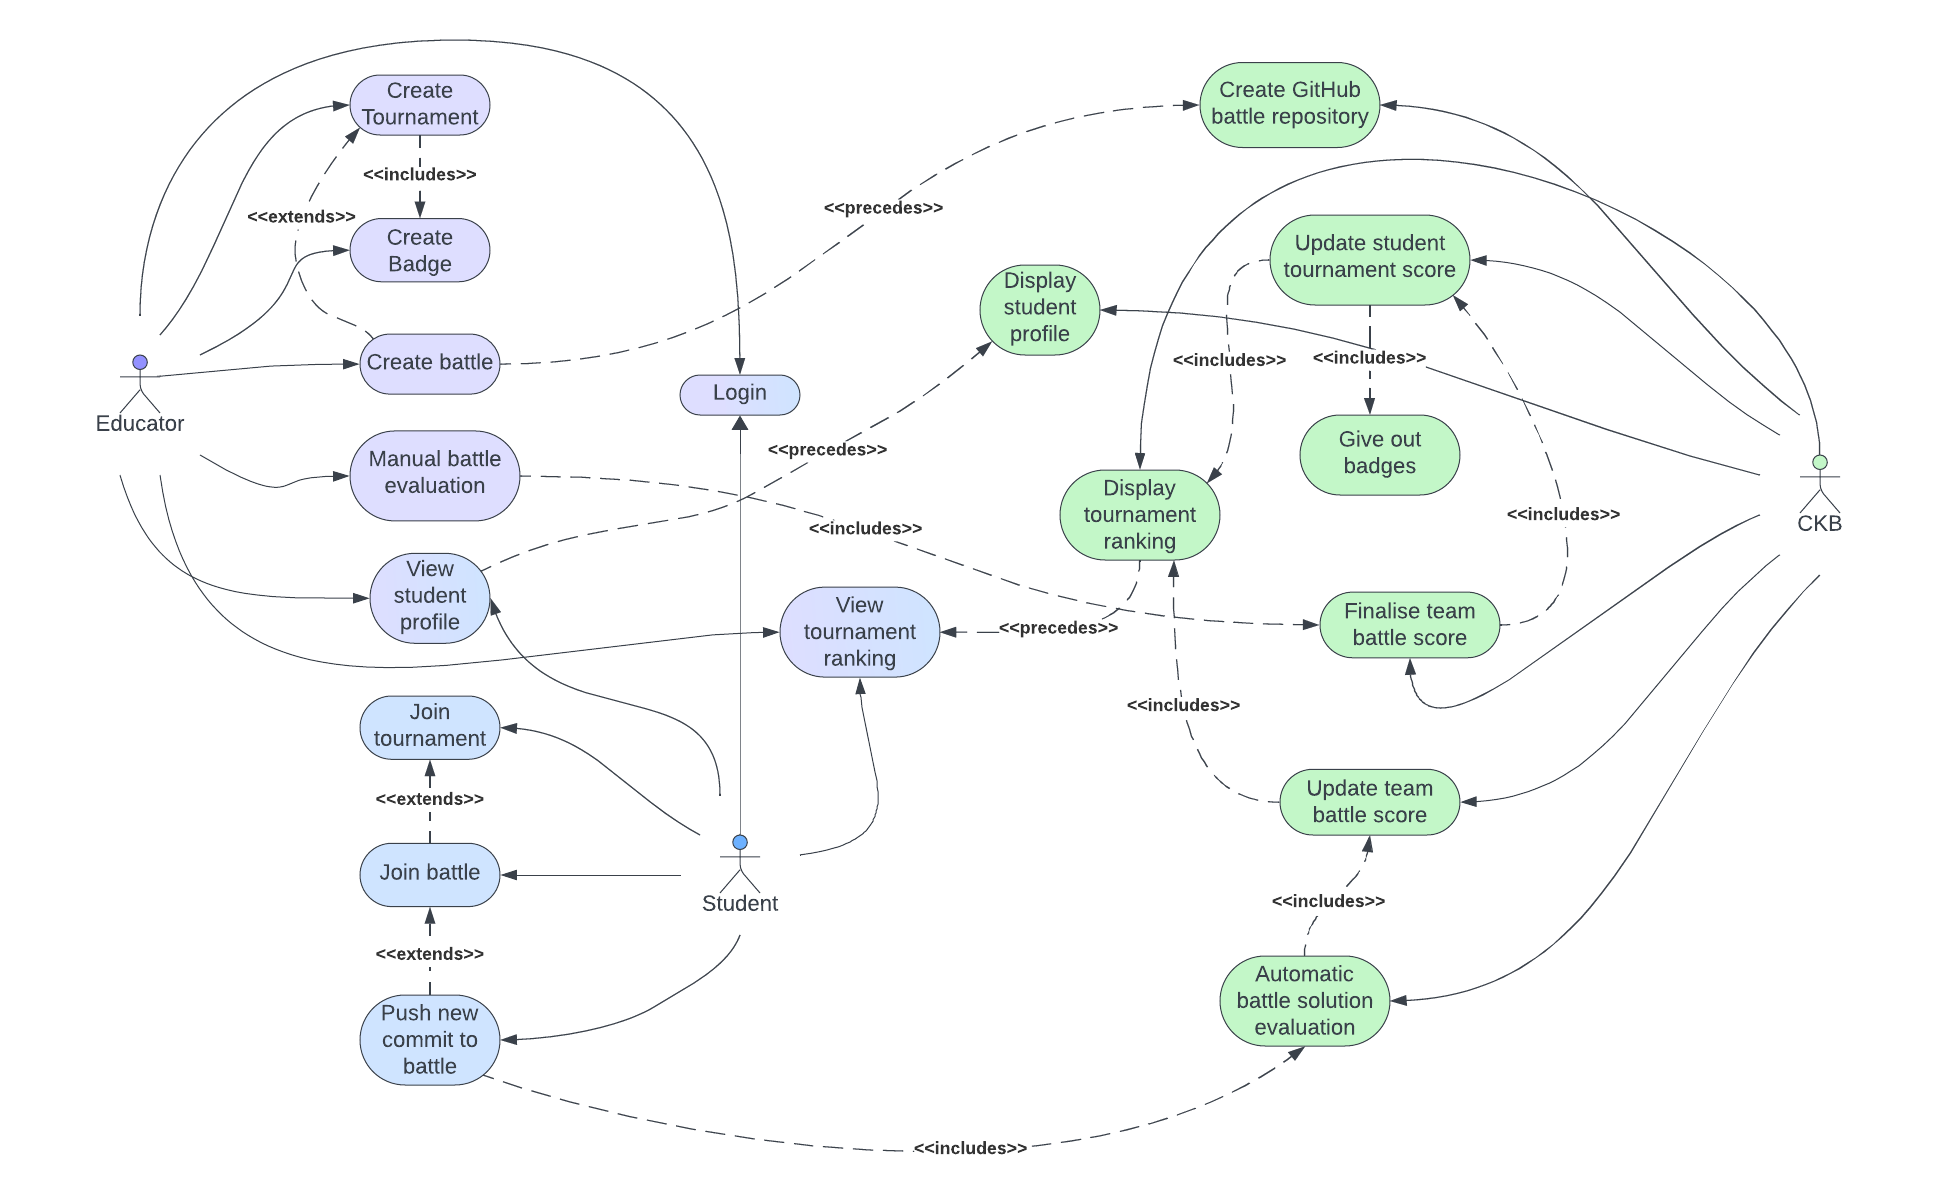
\includegraphics[width=\textwidth]{Graphics/Use case diagram.png}
\caption{Use case diagram.}
\label{fig:use case diagram}
\end{figure}

\clearpage
\newpage





\subsection{Requirements Mapping}
\label{sec:requirements_mapping}

This section maps the functional requirements and domain assumptions to the specific goals of the CodeKataBattle project. This mapping ensures that each goal is achievable through the fulfillment of certain requirements under the given assumptions.

\subsection{Goals to Requirements and Domain Assumptions}


% Goal 1
\begin{longtable}{|p{0.5\textwidth}|p{0.5\textwidth}|}
\hline
\multicolumn{2}{|c|}{\begin{minipage}{0.9\textwidth}
\centering
\vspace{5pt}
\textbf{[G2] Enable Educators to set up test-driven coding challenges including automated feedback online}
\vspace{5pt}
\end{minipage}} \\
\hline
\textbf{Requirements} & \textbf{Domain Assumptions} \\
\hline
R3-R5 Tournament creation with badges & D4 Educators' understanding of version control \\
R8-R13 Battle setup with technical documents and deadlines & D5 Correct automated testing scripts \\
R19 Manual scoring option for educators & R27 Boolean expressions for badge rules \\
\hline
\end{longtable}

% Goal 2
\begin{longtable}{|p{0.5\textwidth}|p{0.5\textwidth}|}
\hline
\multicolumn{2}{|c|}{\begin{minipage}{0.9\textwidth}
\centering
\vspace{5pt}
\textbf{[G2] Enable Educators to set up test-driven coding challenges including automated feedback online}
\vspace{5pt}
\end{minipage}} \\
\hline
\textbf{Requirements} & \textbf{Domain Assumptions} \\
\hline
R3-R5 Tournament creation with badges & D4 Educators' understanding of version control \\
R8-R13 Battle setup with technical documents and deadlines & D5 Correct automated testing scripts \\
R19 Manual scoring option for educators & R27 Boolean expressions for badge rules \\
\hline
\end{longtable}


% Goal 3
\begin{longtable}{|p{0.5\textwidth}|p{0.5\textwidth}|}
\hline
\multicolumn{2}{|c|}{\begin{minipage}{0.9\textwidth}
\centering
\vspace{5pt}
\textbf{[G3] Simulate a Real-world software development scenario through the use of GitHub and GitHub Actions.}
\vspace{5pt}
\end{minipage}} \\
\hline
\textbf{Requirements} & \textbf{Domain Assumptions} \\
\hline
R15 Use of GitHub repositories for code katas & D10 Compatibility with code kata requirements \\
R17 Timeliness evaluation of submissions & D13 Adherence to test-first development approach \\
\hline
\end{longtable}

% Goal 4
\begin{longtable}{|p{0.5\textwidth}|p{0.5\textwidth}|}
\hline
\multicolumn{2}{|c|}{\begin{minipage}{0.9\textwidth}
\centering
\vspace{5pt}
\textbf{[G4] Enable Educators to set up test-driven coding challenges including automated feedback online}
\vspace{5pt}
\end{minipage}} \\
\hline
\textbf{Requirements} & \textbf{Domain Assumptions} \\
\hline
R22 Update of personal tournament scores & D14 Use of scores for constructive feedback \\
R23 Maintenance of visible tournament rank & D15 Fair use of the platform by users \\
R28-R30 Performance visualization tools &  \\
\hline
\end{longtable}

\subsection{Sequence Diagrams}

\begin{figure}[Htbp!]
    \centering
    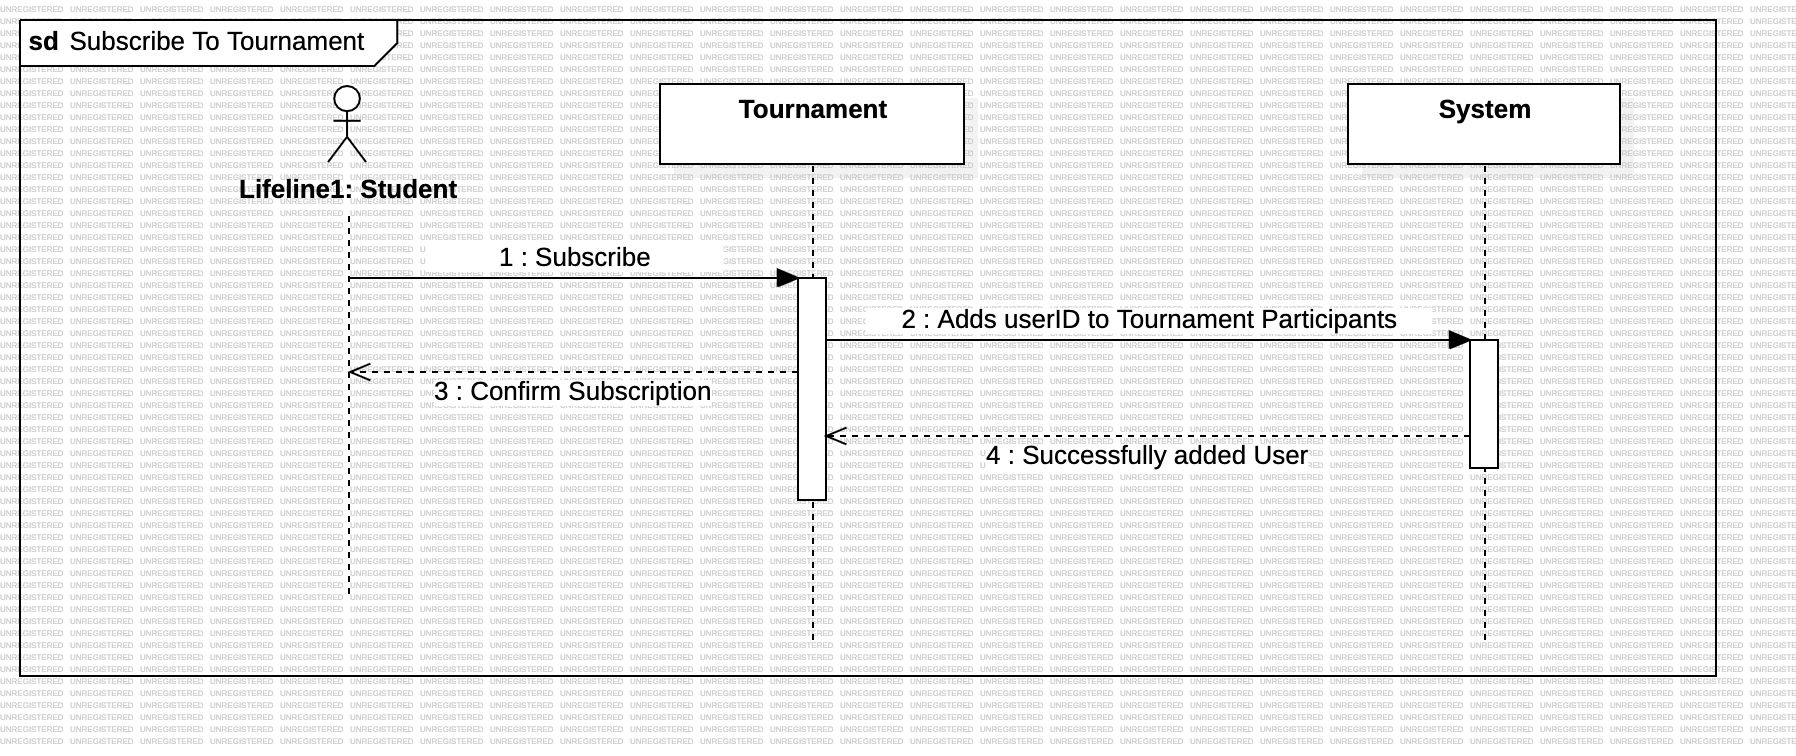
\includegraphics[width=\textwidth]{Graphics/Sequence Diagrams/SubscribeToTournament.png}
    \caption{Sequence Diagram: Subscribe to Tournament}
    \label{fig:Subscribe}
\end{figure}


\begin{figure}[Htbp!]
    \centering
    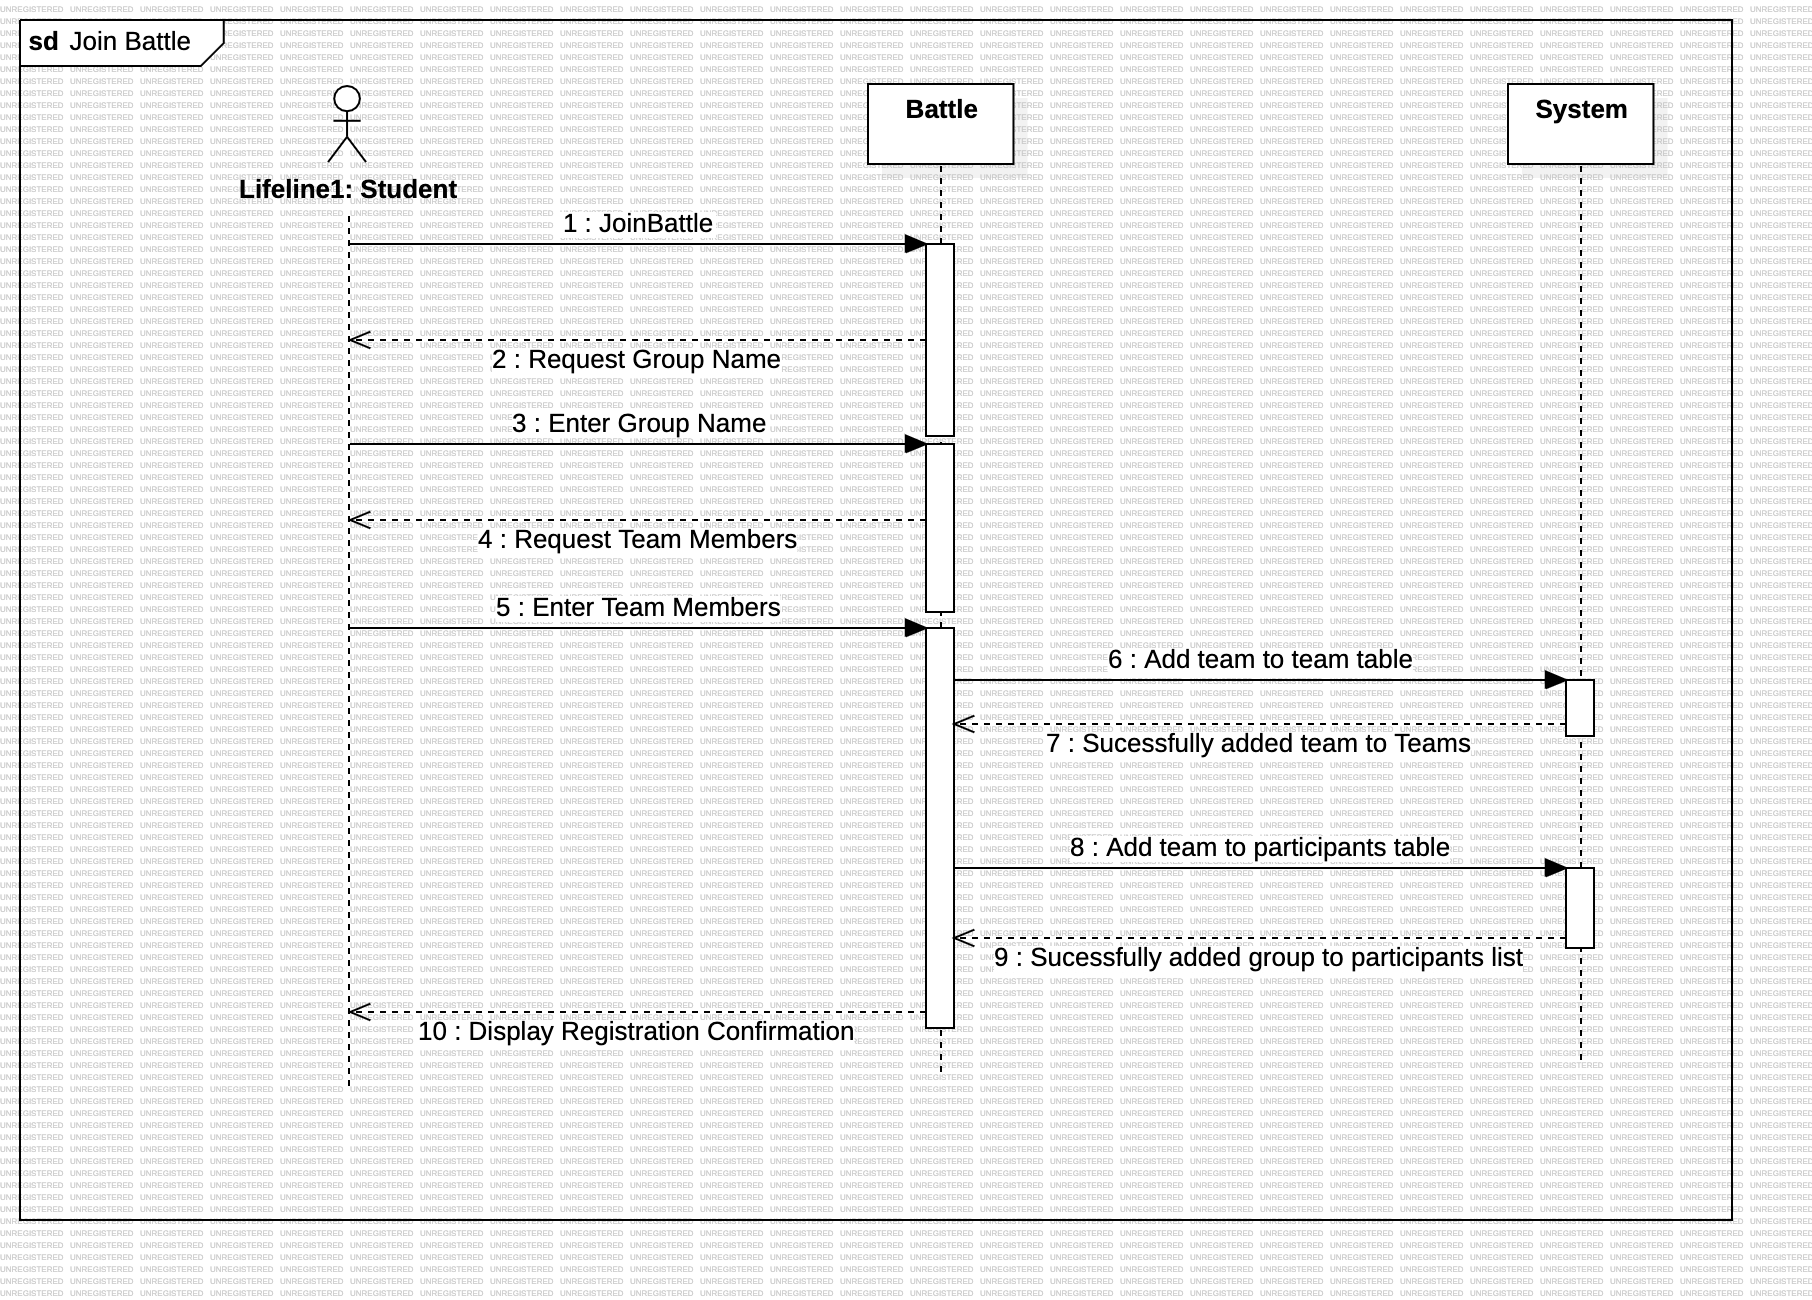
\includegraphics[width=\textwidth]{Graphics/Sequence Diagrams/Join Battle.png}
    \caption{Sequence Diagram: Join Battle}
    \label{fig:Join}
\end{figure}

\newpage

\begin{figure}[Htbp!]
    \centering
    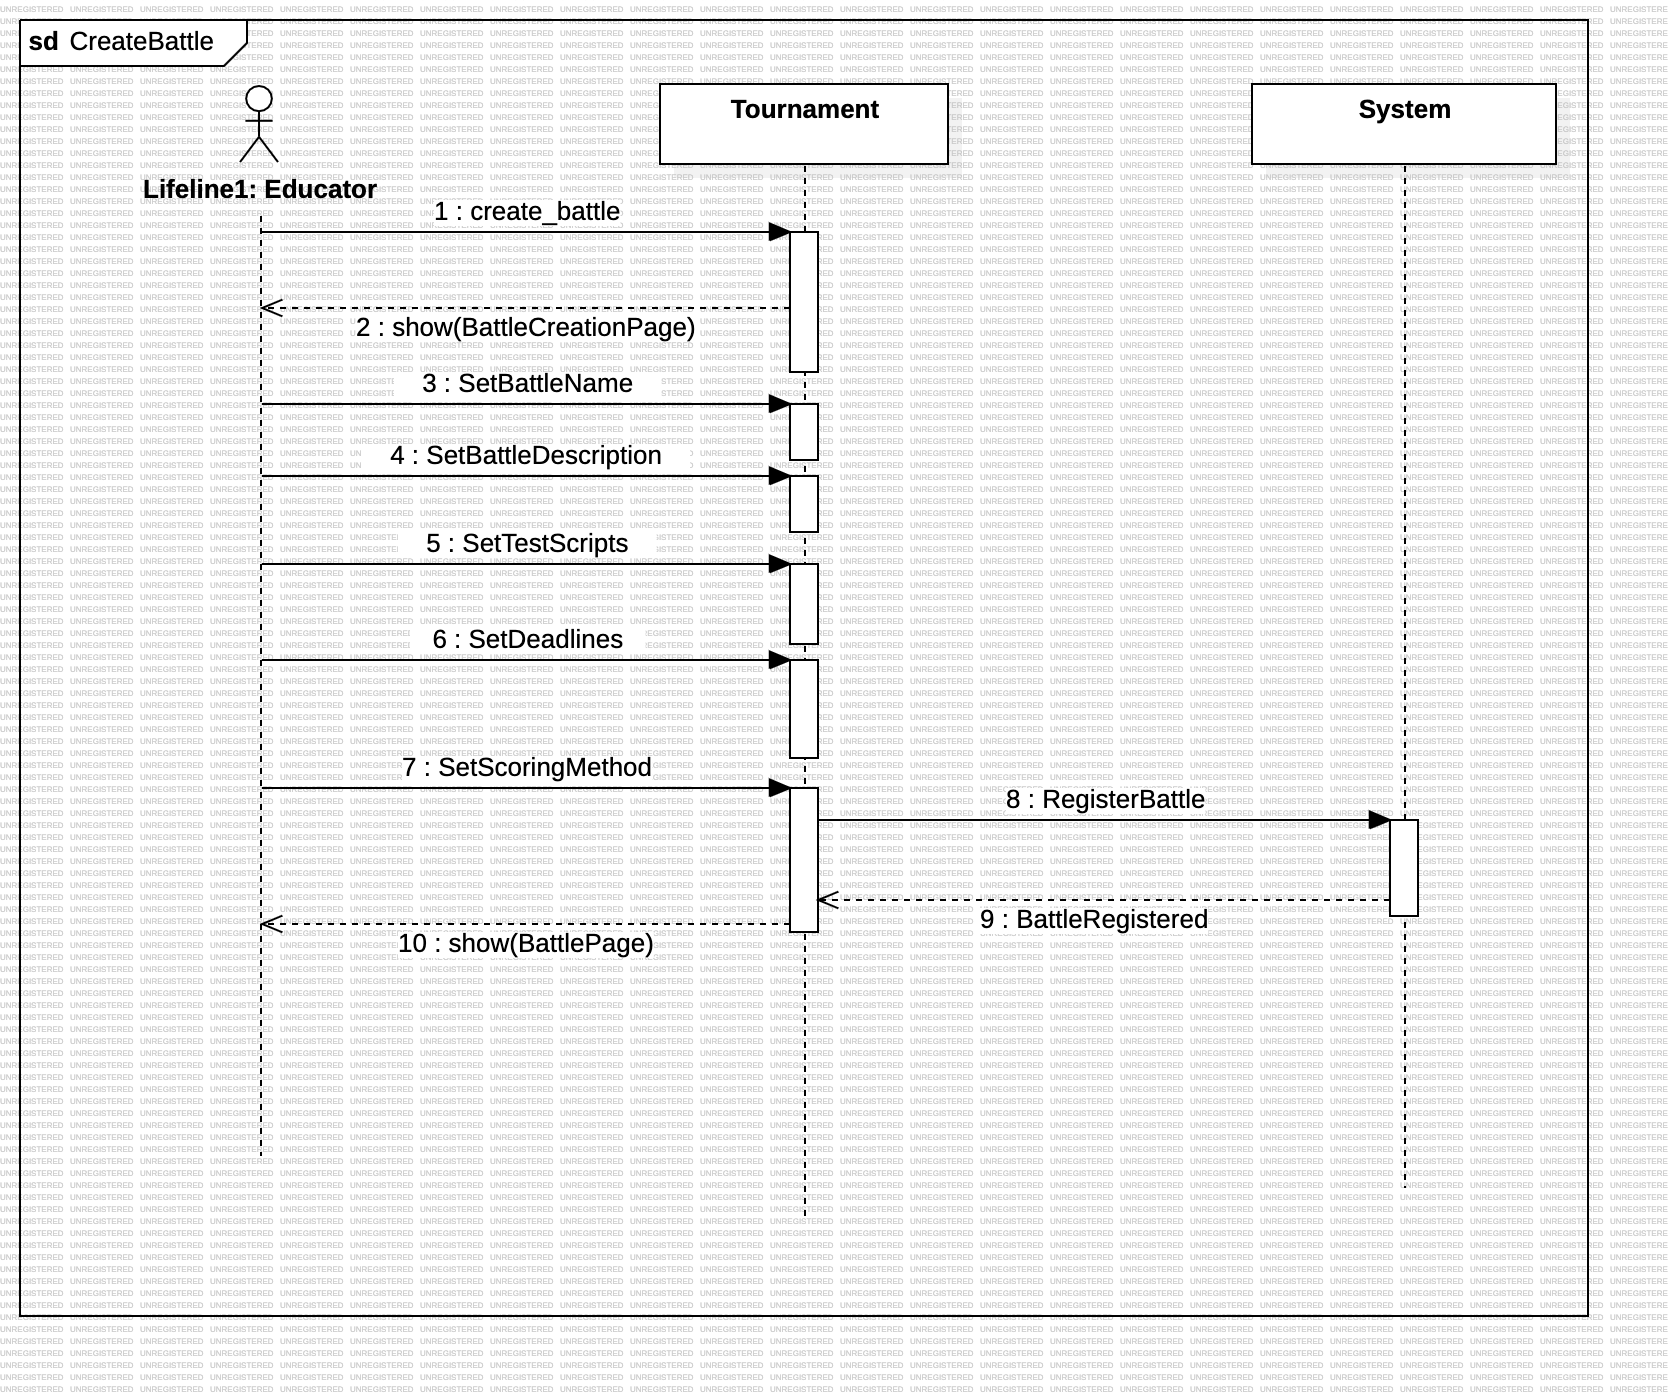
\includegraphics[width=\textwidth]{Graphics/Sequence Diagrams/CreateBattle.png}
    \caption{Sequence Diagram: Create Battle}
    \label{fig:CreateBattle}
\end{figure}



\begin{figure}[Htbp!]
    \centering
    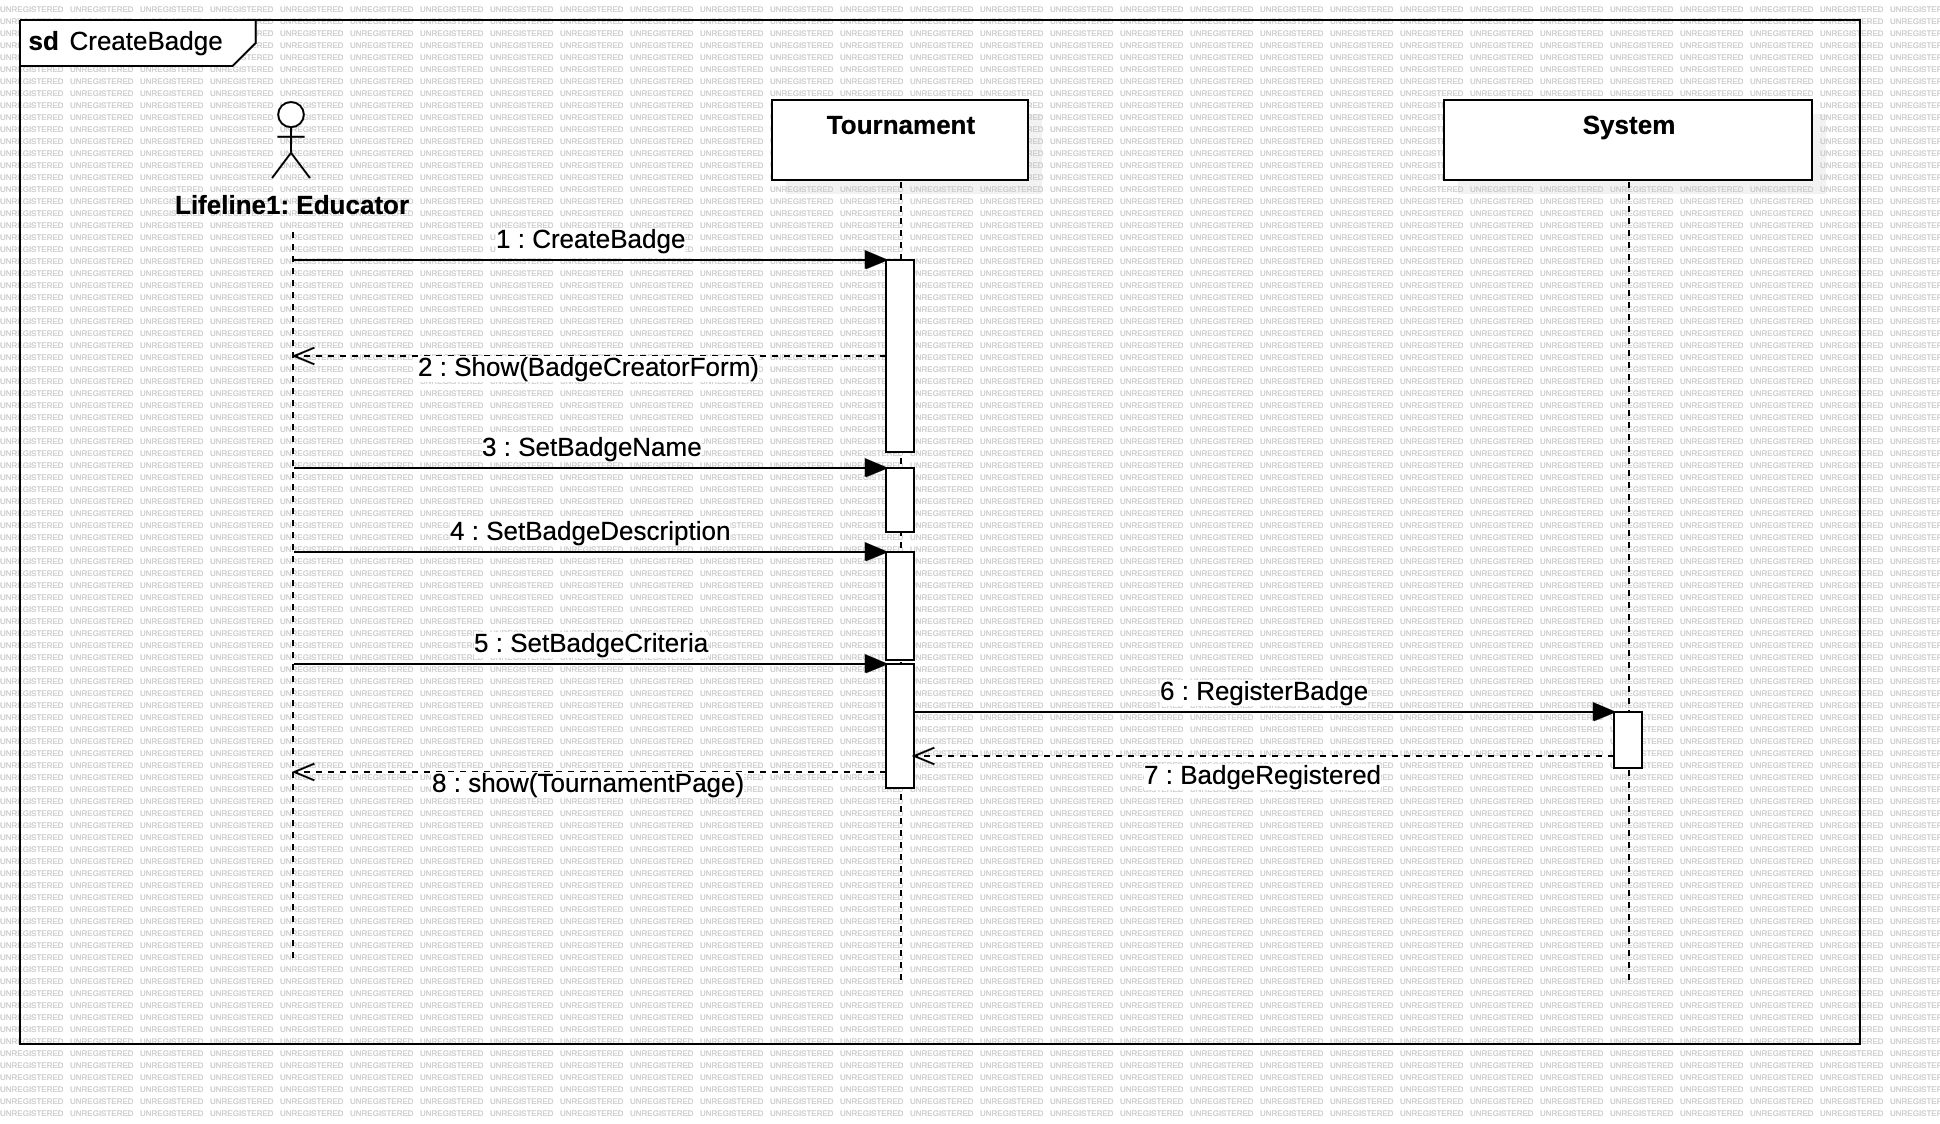
\includegraphics[width=\textwidth]{Graphics/Sequence Diagrams/CreateBadge.png}
    \caption{Sequence Diagram: Create Badge}
    \label{fig:CreateBadge}
\end{figure}
\newpage

\begin{figure}[Htbp!]
    \centering
    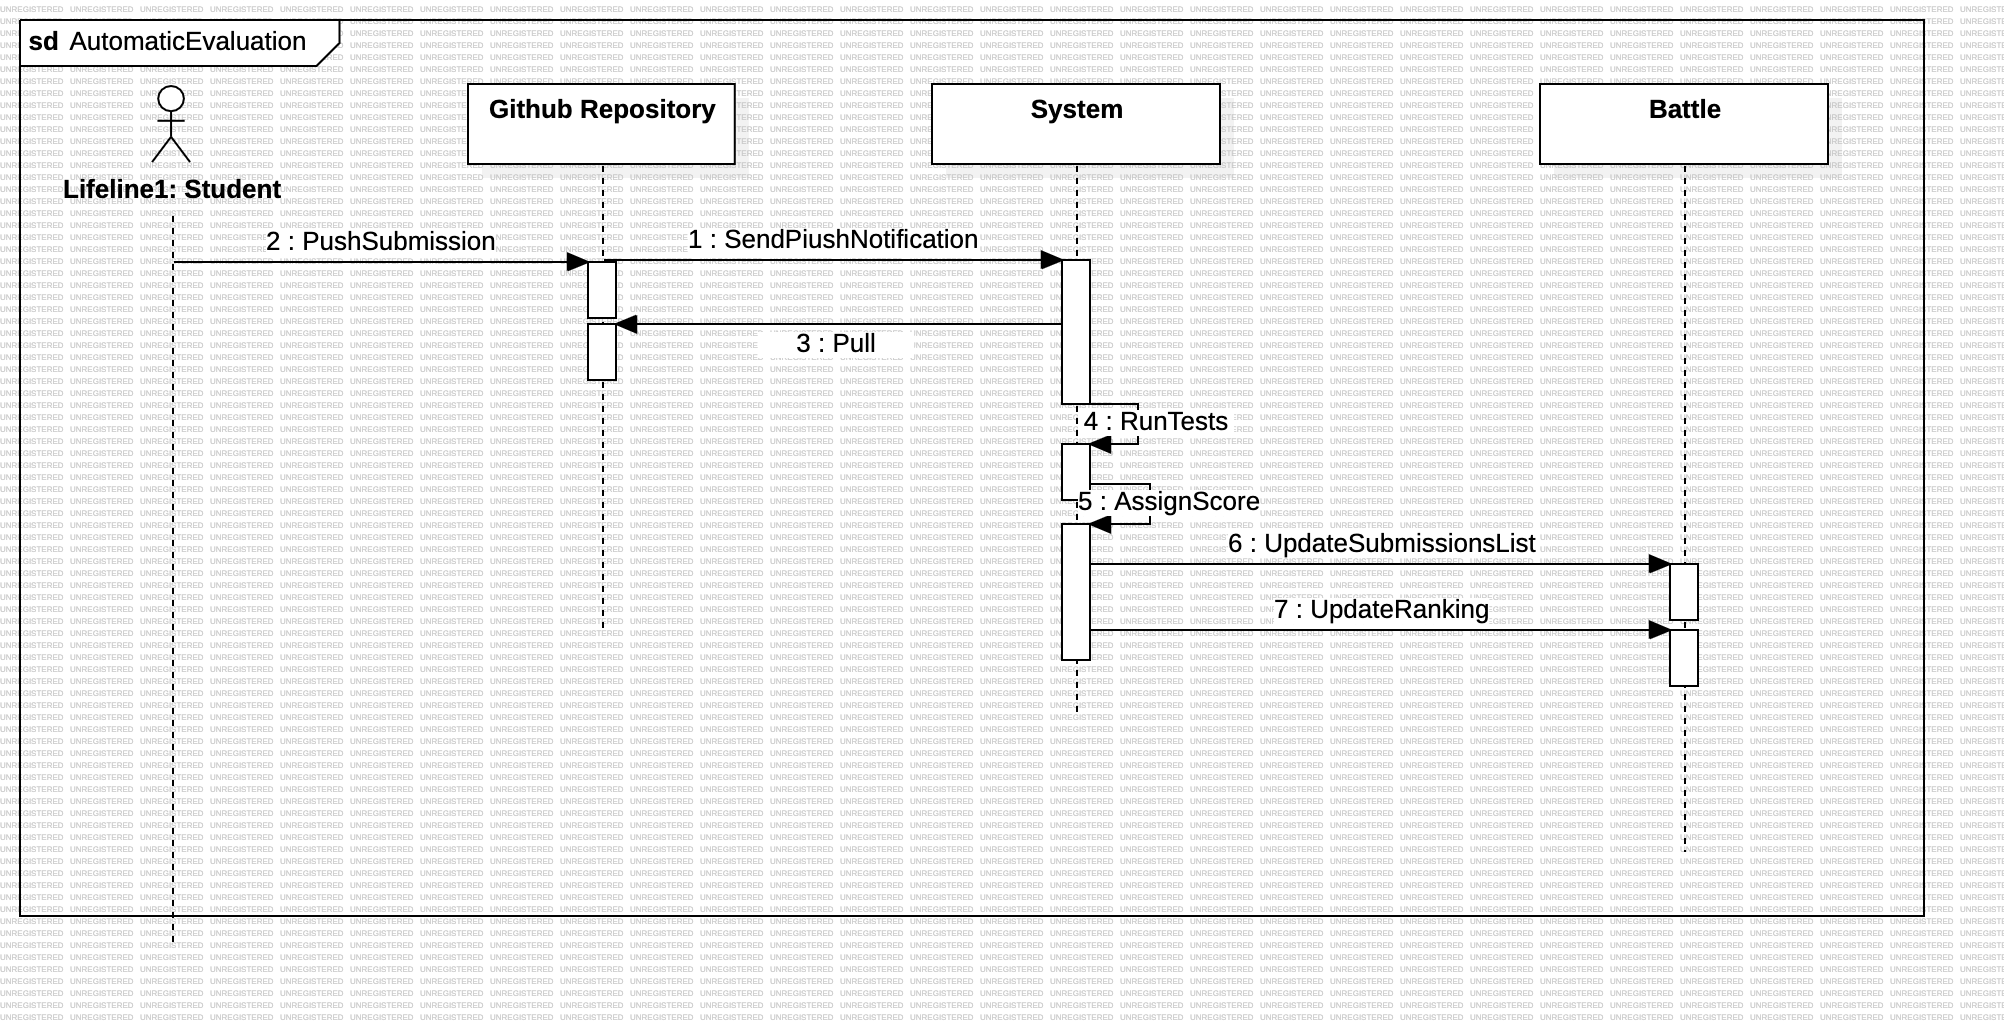
\includegraphics[width=\textwidth]{Graphics/Sequence Diagrams/AutomaticEvaluation.png}
    \caption{Sequence Diagram: Automatic Evaluation}
    \label{fig:AutoEval}
\end{figure}


\begin{figure}[Htbp!]
    \centering
    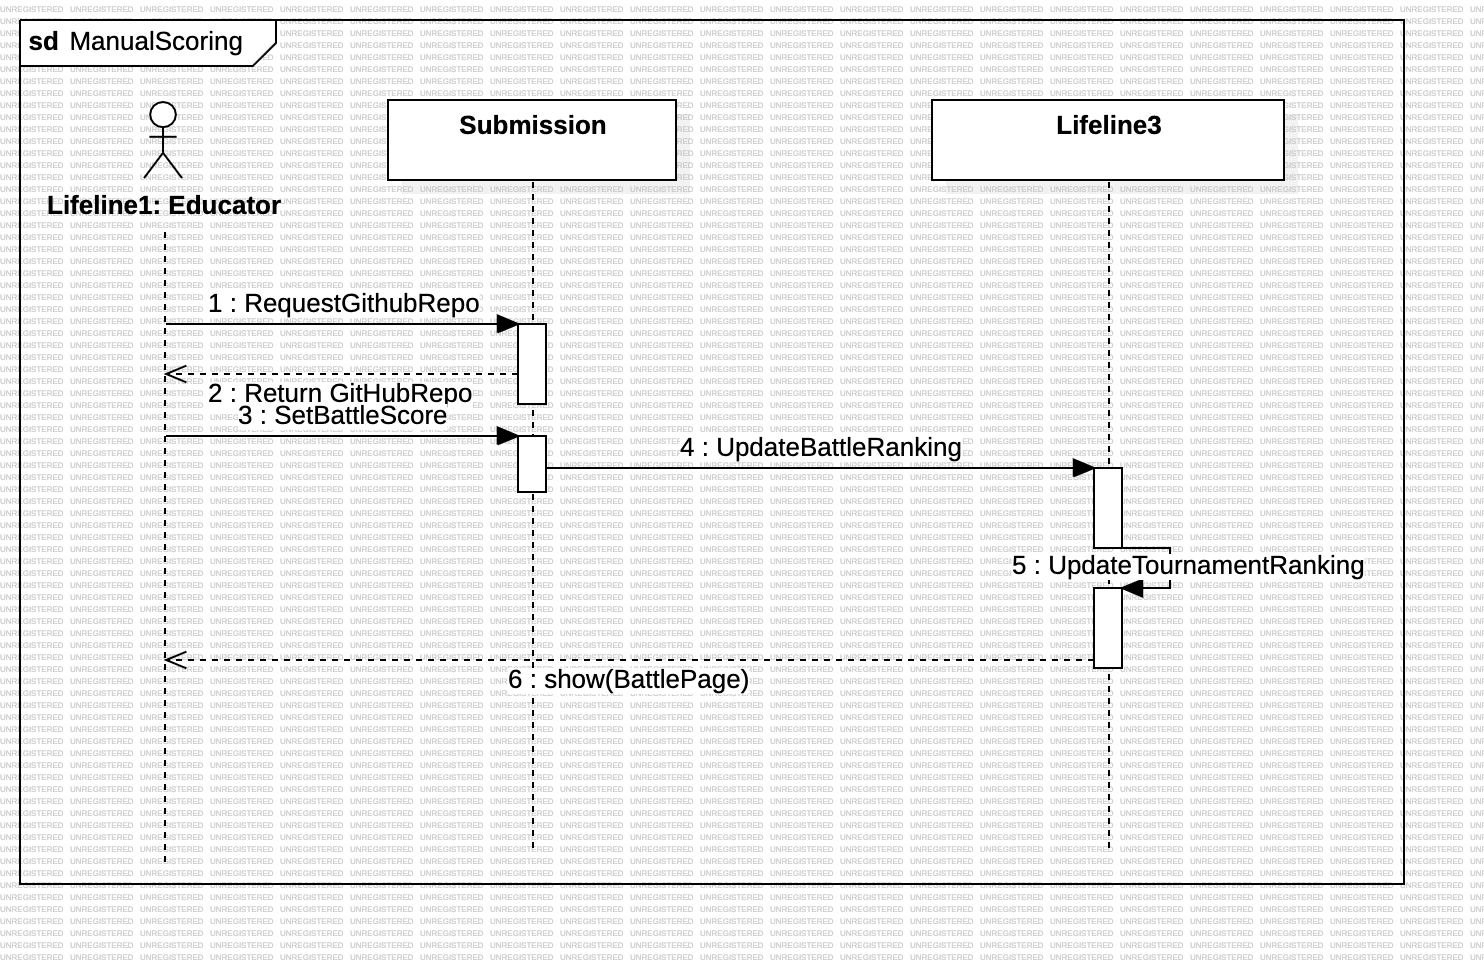
\includegraphics[width=\textwidth]{Graphics/Sequence Diagrams/ManualScoring.png}
    \caption{Sequence Diagram: Manual Evaluation }
    \label{fig:ManEval}
\end{figure}

\newpage
\begin{figure}[Htbp!]
    \centering
    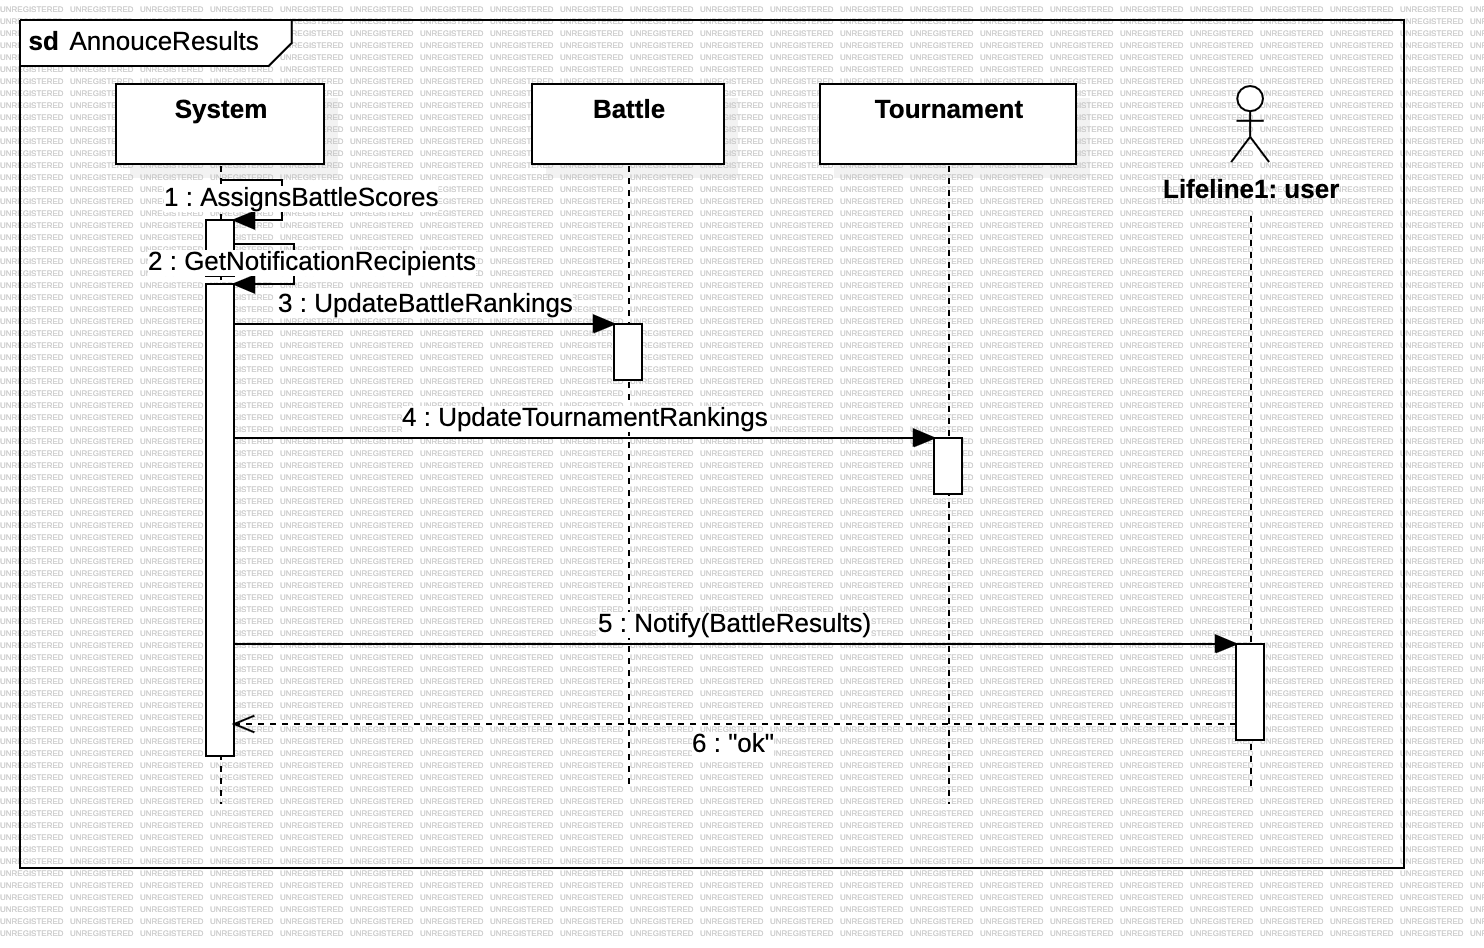
\includegraphics[width=\textwidth]{Graphics/Sequence Diagrams/AnnouceResults.png}
    \caption{Sequence Diagram: Announce Battle Results}
    \label{fig:Announcement}
\end{figure}



\begin{figure}[Htbp!]
    \centering
    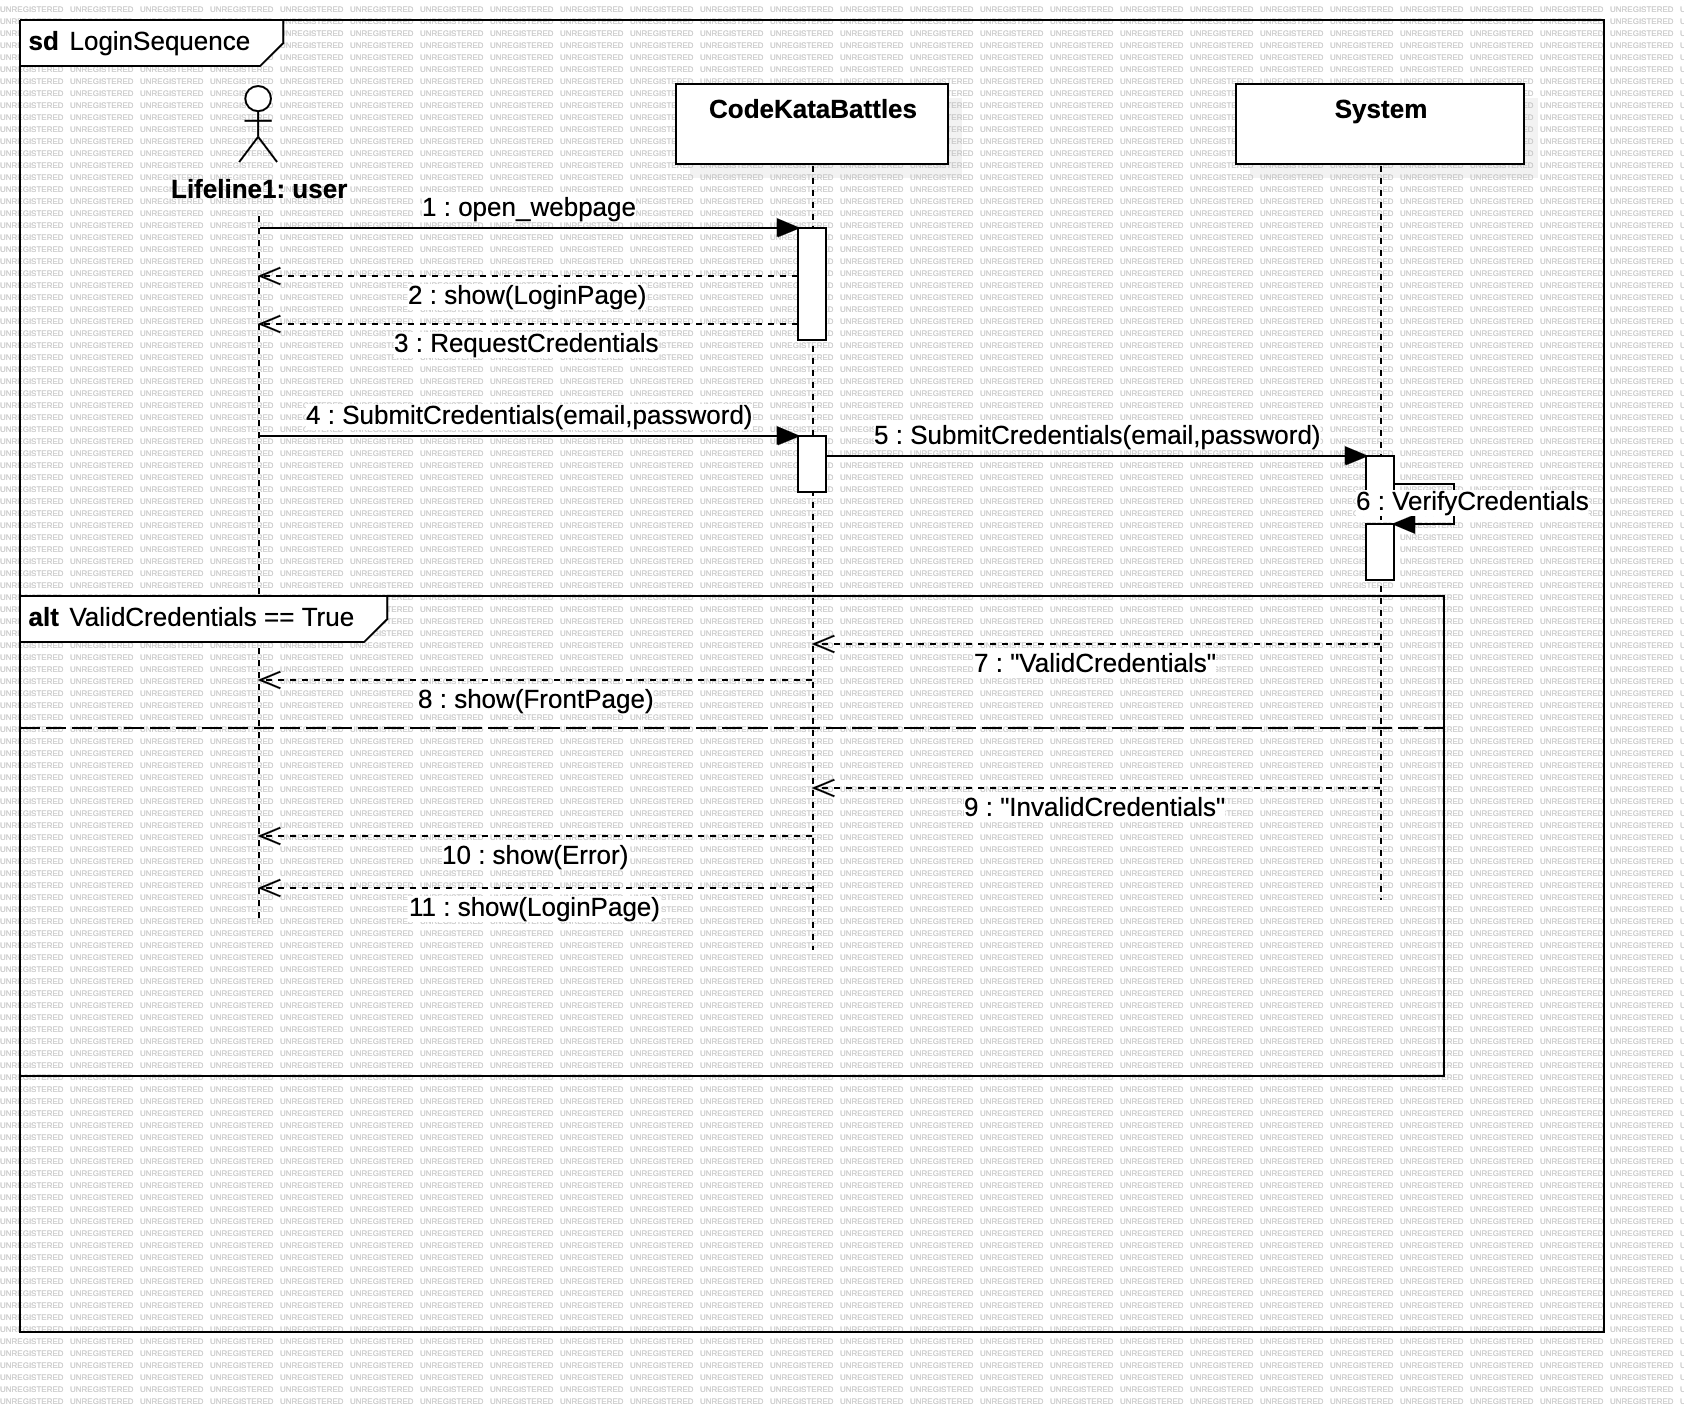
\includegraphics[width=\textwidth]{Graphics/Sequence Diagrams/LoginSequence.png}
    \caption{Sequence Diagram: Log-in Sequence}
    \label{fig:login}
\end{figure}

\newpage
\clearpage
\newpage
\section{Formal Analysis Using Alloy}
\label{sec:Alloy}


\begin{figure}[htbp!]
    \centering
    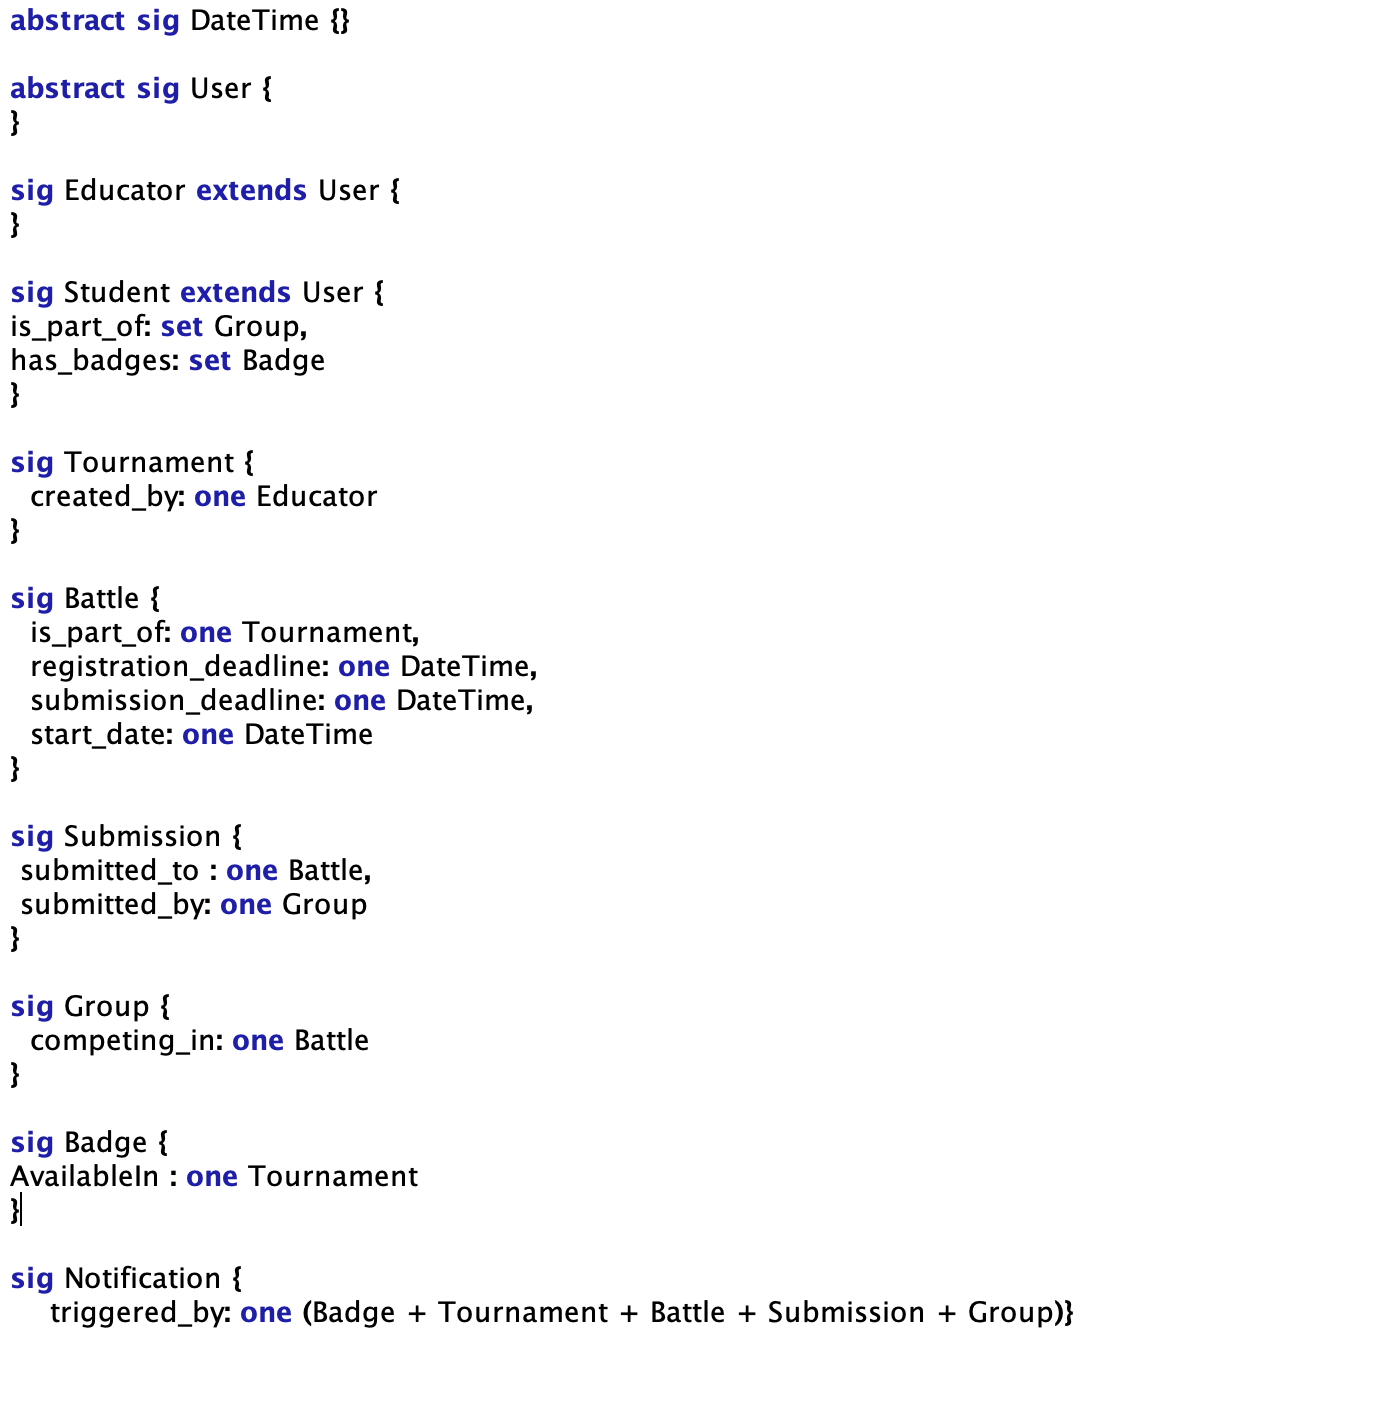
\includegraphics[width=\textwidth]{Graphics/Alloy/Sigs.png}
    \caption{Sigs}
    \label{fig:sigs}
\end{figure}

\begin{figure}[htbp!]
    \centering
    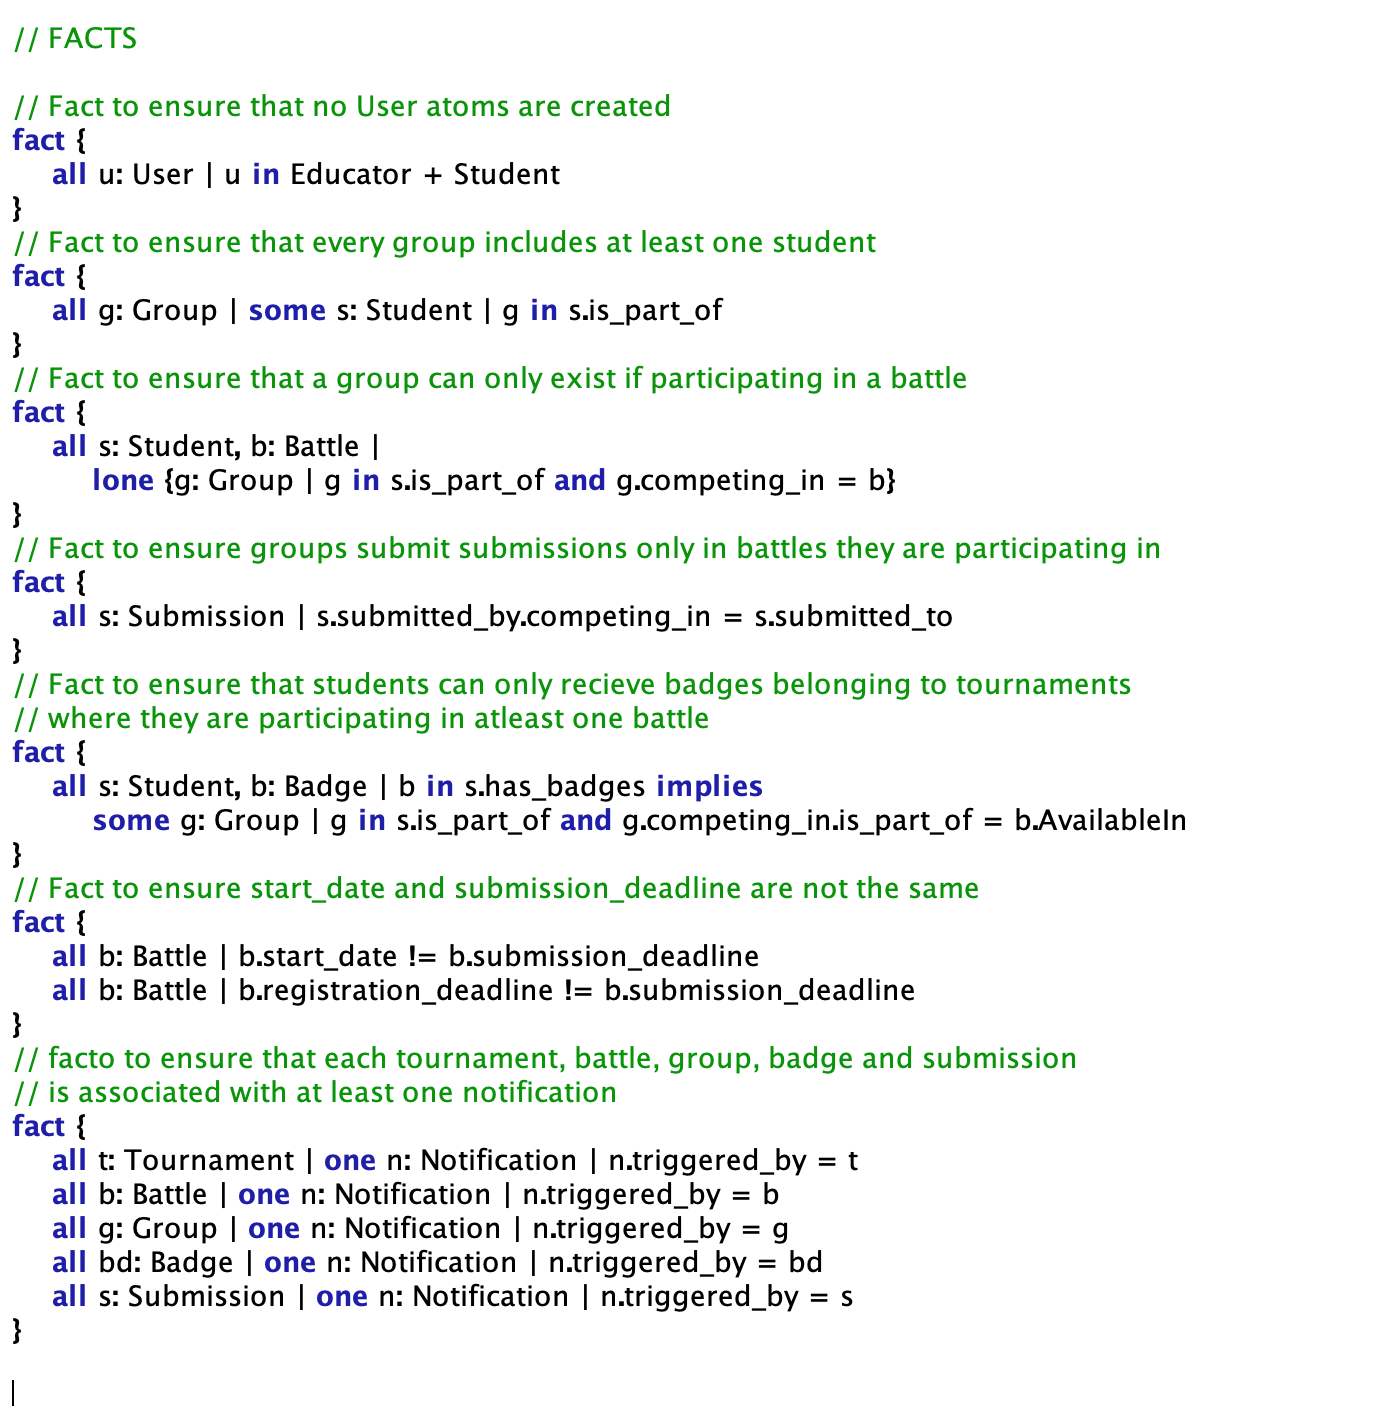
\includegraphics[width=\textwidth]{Graphics/Alloy/Facts.png}
    \caption{Facts}
    \label{fig:Facts}
\end{figure}


\begin{figure}[htbp!]
    \centering
    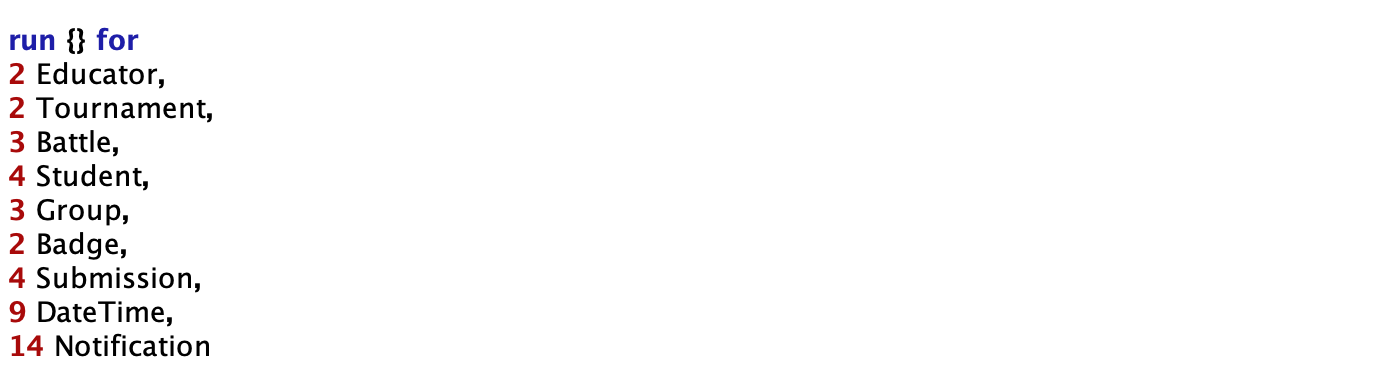
\includegraphics[width=\textwidth]{Graphics/Alloy/Run.png}
    \caption{Run Command}
    \label{fig:runcommand}
\end{figure}


\begin{figure}[htbp!]
    \centering
    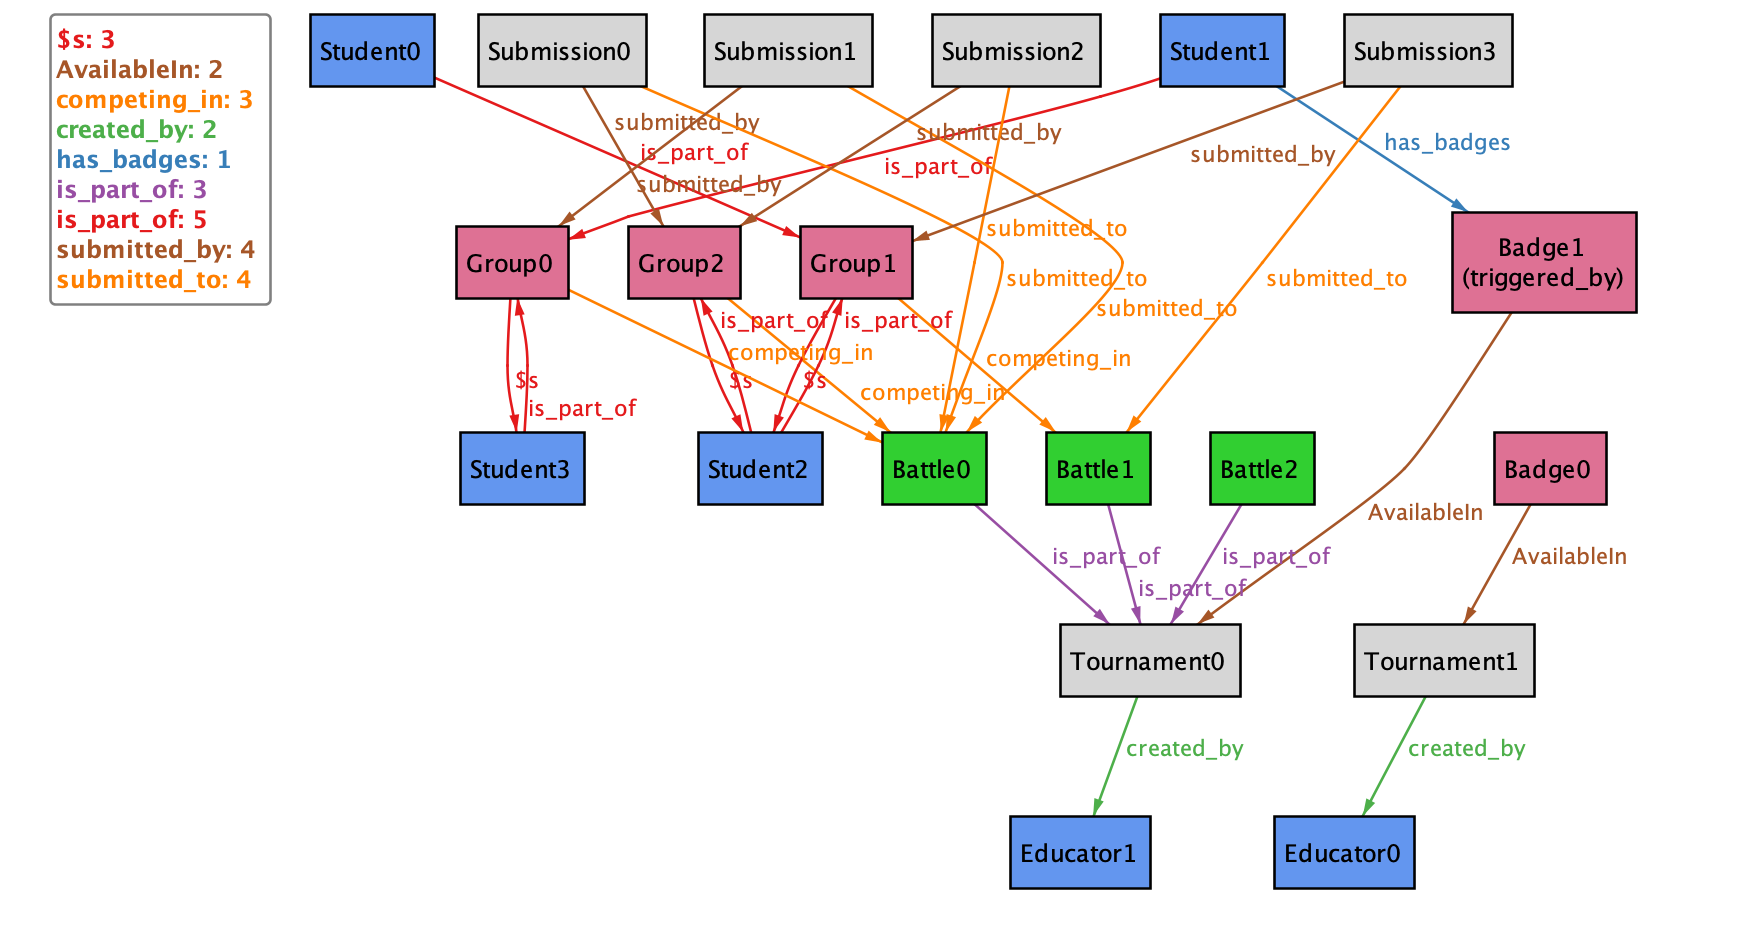
\includegraphics[width=\textwidth]{Graphics/Alloy/Alloy.png}
    \caption{Example}
    \label{fig:example}
\end{figure}

\newpage
\clearpage
\newpage
\section{Efforts Spent}
\label{sec:effort}
The tables below indicate how much time each participant has spent on each of the sections in the report. 

\subsection{Karl Kieler}
\begin{table}[h]
\centering
\begin{tabular}{|c|c|}
\hline
Section & Time Spent (Hours) \\ \hline
Introduction & 2 \\ \hline
Overall Description & 11 \\ \hline
Specific Requirements & 16 \\ \hline
Formal Analysis & 12 \\ \hline
\end{tabular}
\end{table}


\subsection{Leonie Dragun}
\begin{table}[h]
\centering
\begin{tabular}{|c|c|}
\hline
Section & Time Spent (Hours) \\ \hline
Introduction & 4 \\ \hline
Overall Description & 12 \\ \hline
Specific Requirements & 16 \\ \hline
Formal Analysis & 12\\ \hline
\end{tabular}
\end{table}


\subsection{Aske Schytt Meineche}
\begin{table}[h]
\centering
\begin{tabular}{|c|c|}
\hline
Section & Time Spent (Hours) \\ \hline
Introduction & 4 \\ \hline
Overall Description & 9 \\ \hline
Specific Requirements & 19 \\ \hline
Formal Analysis & 12 \\ \hline
\end{tabular}
\end{table}

\newpage
\section{References}
\label{sec:ref}

\begin{enumerate}
    \item Diagrams made with: StarUML and Microsoft PowerPoint
    \item Mockups made with Microsoft PowerPoint
\end{enumerate}




%\bibliography{refs}

\end{document}
